% Options for packages loaded elsewhere
\PassOptionsToPackage{unicode}{hyperref}
\PassOptionsToPackage{hyphens}{url}
\PassOptionsToPackage{dvipsnames,svgnames,x11names}{xcolor}
\documentclass[
  french,
  10pt,
  a4paper,
]{article}
\usepackage{xcolor}
\usepackage[margin=2.2cm]{geometry}
\usepackage{amsmath,amssymb}
\setcounter{secnumdepth}{-\maxdimen} % remove section numbering
\usepackage{iftex}
\ifPDFTeX
  \usepackage[T1]{fontenc}
  \usepackage[utf8]{inputenc}
  \usepackage{textcomp} % provide euro and other symbols
\else % if luatex or xetex
  \usepackage{unicode-math} % this also loads fontspec
  \defaultfontfeatures{Scale=MatchLowercase}
  \defaultfontfeatures[\rmfamily]{Ligatures=TeX,Scale=1}
\fi
\usepackage{lmodern}
\ifPDFTeX\else
  % xetex/luatex font selection
\fi
% Use upquote if available, for straight quotes in verbatim environments
\IfFileExists{upquote.sty}{\usepackage{upquote}}{}
\IfFileExists{microtype.sty}{% use microtype if available
  \usepackage[]{microtype}
  \UseMicrotypeSet[protrusion]{basicmath} % disable protrusion for tt fonts
}{}
\makeatletter
\@ifundefined{KOMAClassName}{% if non-KOMA class
  \IfFileExists{parskip.sty}{%
    \usepackage{parskip}
  }{% else
    \setlength{\parindent}{0pt}
    \setlength{\parskip}{6pt plus 2pt minus 1pt}}
}{% if KOMA class
  \KOMAoptions{parskip=half}}
\makeatother
\usepackage{longtable,booktabs,array}
\usepackage{calc} % for calculating minipage widths
% Correct order of tables after \paragraph or \subparagraph
\usepackage{etoolbox}
\makeatletter
\patchcmd\longtable{\par}{\if@noskipsec\mbox{}\fi\par}{}{}
\makeatother
% Allow footnotes in longtable head/foot
\IfFileExists{footnotehyper.sty}{\usepackage{footnotehyper}}{\usepackage{footnote}}
\makesavenoteenv{longtable}
\ifLuaTeX
\usepackage[bidi=basic,shorthands=off,]{babel}
\else
\usepackage[bidi=default,shorthands=off,]{babel}
\fi
\ifLuaTeX
  \usepackage{selnolig} % disable illegal ligatures
\fi
\setlength{\emergencystretch}{3em} % prevent overfull lines
\providecommand{\tightlist}{%
  \setlength{\itemsep}{0pt}\setlength{\parskip}{0pt}}
% Fichier LaTeX généré par docs/build/build_pdf.sh à partir de README.md.
% Compilation (depuis le dossier de ce fichier), deux fois pour la table des matières :
%   pdflatex 01_README.tex
% Chaque image est un bloc \begin{figure} ... \includegraphics{fichier} ... \end{figure}.
% Pour mettre votre capture : changez seulement le nom du fichier dans \includegraphics{...}
% (chemin relatif à ce dossier, par exemple ../images/guides/ma_capture.png), puis recompilez.
% Tant que le fichier est absent, un cadre « CAPTURE À INSÉRER » s'affiche à sa place.
\newcommand{\CredixShortTitle}{README CREDIX}
% Préambule commun aux PDF du dossier de remise CREDIX (compilé avec pdfLaTeX via pandoc)
\usepackage[scaled=.92]{helvet}
\renewcommand{\familydefault}{\sfdefault}
\usepackage{pifont}
\usepackage{amssymb}
% Caractères Unicode utilisés dans les documents (pdfLaTeX ne les connaît pas d'office)
\DeclareUnicodeCharacter{03C1}{\ensuremath{\rho}}
\DeclareUnicodeCharacter{2265}{\ensuremath{\geq}}
\DeclareUnicodeCharacter{2264}{\ensuremath{\leq}}
\DeclareUnicodeCharacter{2248}{\ensuremath{\approx}}
\DeclareUnicodeCharacter{2192}{\ensuremath{\rightarrow}}
\DeclareUnicodeCharacter{2190}{\ensuremath{\leftarrow}}
\DeclareUnicodeCharacter{2212}{\ensuremath{-}}
\DeclareUnicodeCharacter{2713}{\ding{51}}
\DeclareUnicodeCharacter{2714}{\ding{52}}
\DeclareUnicodeCharacter{2717}{\ding{55}}
\DeclareUnicodeCharacter{25B2}{\ensuremath{\blacktriangle}}
\DeclareUnicodeCharacter{25CB}{\ensuremath{\circ}}
\DeclareUnicodeCharacter{2500}{-}
\DeclareUnicodeCharacter{2502}{|}
\DeclareUnicodeCharacter{250C}{+}
\DeclareUnicodeCharacter{2510}{+}
\DeclareUnicodeCharacter{2514}{+}
\DeclareUnicodeCharacter{2518}{+}
\DeclareUnicodeCharacter{251C}{+}
\DeclareUnicodeCharacter{2524}{+}
\DeclareUnicodeCharacter{252C}{+}
\DeclareUnicodeCharacter{2534}{+}
\DeclareUnicodeCharacter{253C}{+}
\DeclareUnicodeCharacter{0192}{\textit{f}}
\DeclareUnicodeCharacter{2011}{-}
\DeclareUnicodeCharacter{202F}{\,}
\DeclareUnicodeCharacter{2009}{\,}
\DeclareUnicodeCharacter{00D7}{\ensuremath{\times}}
\DeclareUnicodeCharacter{25A0}{\ensuremath{\blacksquare}}
\DeclareUnicodeCharacter{2022}{\ensuremath{\bullet}}
\DeclareUnicodeCharacter{2026}{\ldots}
\DeclareUnicodeCharacter{2460}{\ding{172}}
\DeclareUnicodeCharacter{2461}{\ding{173}}
\DeclareUnicodeCharacter{2462}{\ding{174}}
\DeclareUnicodeCharacter{2463}{\ding{175}}
\DeclareUnicodeCharacter{2464}{\ding{176}}
\DeclareUnicodeCharacter{2465}{\ding{177}}
\DeclareUnicodeCharacter{2466}{\ding{178}}
\DeclareUnicodeCharacter{2467}{\ding{179}}
\usepackage{fvextra}
\DefineVerbatimEnvironment{verbatim}{Verbatim}{breaklines=true,breakanywhere=true,fontsize=\footnotesize,frame=single,framerule=0.3pt,rulecolor=\color[gray]{0.7},framesep=2mm,xleftmargin=1mm,xrightmargin=1mm}
\fvset{breaklines=true,breakanywhere=true}
\usepackage{fancyhdr}
\usepackage{tcolorbox}
\usepackage{colortbl}
\usepackage{enumitem}
\definecolor{credixblue}{HTML}{1F3A5F}
\definecolor{credixgray}{HTML}{5F6B7A}
\definecolor{boxbg}{HTML}{F3F5F8}
\setlength{\emergencystretch}{4em}
\renewcommand{\arraystretch}{1.3}
\setlength{\parindent}{0pt}
\setlength{\parskip}{0.55em}
\setlist{itemsep=0.15em,topsep=0.3em}
\pagestyle{fancy}
\fancyhf{}
\fancyhead[L]{\small\color{credixgray}\textsc{\CredixShortTitle}}
\fancyhead[R]{\small\color{credixgray}CREDIX --- Dossier de remise}
\fancyfoot[C]{\small\color{credixgray}\thepage}
\renewcommand{\headrulewidth}{0.3pt}
\renewcommand{\footrulewidth}{0pt}
\fancypagestyle{plain}{\fancyhf{}\fancyfoot[C]{\small\color{credixgray}\thepage}\renewcommand{\headrulewidth}{0pt}}
\usepackage{titlesec}
\titleformat{\section}{\Large\bfseries\color{credixblue}}{}{0em}{}[\vspace{-0.2em}\color{credixblue}\titlerule]
\titleformat{\subsection}{\large\bfseries\color{credixblue}}{}{0em}{}
\titleformat{\subsubsection}{\normalsize\bfseries\color{credixblue}}{}{0em}{}
% Cadre de repère pour une capture manquante
\newcommand{\CaptureManquante}[2]{%
  \begin{tcolorbox}[colback=boxbg,colframe=credixgray,boxrule=0.5pt,arc=1mm,left=3mm,right=3mm,top=3mm,bottom=3mm,halign=center]
  \textbf{CAPTURE À INSÉRER}\\[0.4em]#1\\[0.4em]{\footnotesize\ttfamily #2}
  \end{tcolorbox}}

% Figures : chaque image est un bloc \begin{figure} ... \includegraphics{fichier} ... \end{figure}.
% Si le fichier est absent, un cadre « CAPTURE À INSÉRER » s'affiche à sa place et la compilation continue.
% Pour mettre votre image : changez seulement le nom du fichier dans \includegraphics{...}.
\usepackage{graphicx}
\usepackage{float}
\usepackage{needspace}
\newcommand{\CredixAlt}{Capture}
\let\CredixOrigIncludegraphics\includegraphics
\renewcommand{\includegraphics}[2][]{%
  \IfFileExists{#2}%
    {\CredixOrigIncludegraphics[#1]{#2}}%
    {\CaptureManquante{\CredixAlt}{\detokenize{#2}}}}
\usepackage{bookmark}
\IfFileExists{xurl.sty}{\usepackage{xurl}}{} % add URL line breaks if available
\urlstyle{same}
\hypersetup{
  pdftitle={CREDIX},
  pdfauthor={SINGHE PENKA Hendrix Donavan},
  pdflang={fr},
  colorlinks=true,
  linkcolor={credixblue},
  filecolor={Maroon},
  citecolor={Blue},
  urlcolor={credixblue},
  pdfcreator={LaTeX via pandoc}}

\author{}
\date{}

\begin{document}

\begin{titlepage}
\thispagestyle{empty}
\centering
\vspace*{3.2cm}
{\color{credixgray}\large\textsc{Projet de fin d'études --- ENSPY, Université de Yaoundé I}\par}
\vspace{2.2cm}
{\Huge\bfseries\color{credixblue} CREDIX\par}
\vspace{0.8cm}
{\Large Guide de récupération, de lancement et de test\par}
\vspace{2cm}
{\color{credixblue}\rule{0.5\linewidth}{0.8pt}\par}
\vspace{1.2cm}
{\large SINGHE PENKA Hendrix Donavan\par}
{\color{credixgray}Dépôt GitHub : HendrixPenka2/credix\par}
\vfill
{\color{credixgray}\small Version du 19/09/2026\par}
\end{titlepage}


\renewcommand*\contentsname{Table des matières}
{
\setcounter{tocdepth}{2}
\tableofcontents
}
\section{CREDIX : système intelligent de scoring du risque de
crédit}\label{credix--systuxe8me-intelligent-de-scoring-du-risque-de-cruxe9dit}

\textbf{Guide complet : comprendre, récupérer, lancer, tester et
modifier le projet.}

Projet de fin d\textquotesingle études (ENSPY, Université de Yaoundé I).
Dépôt GitHub : \url{https://github.com/HendrixPenka2/credix}

\subsection{Comment lire ce guide}\label{comment-lire-ce-guide}

\begin{itemize}
\tightlist
\item
  \textbf{Si vous voulez seulement lancer le projet}, allez directement
  aux sections 3 à 7, dans l\textquotesingle ordre. Chaque étape suppose
  que la précédente a réussi.
\item
  Les blocs gris sont des \textbf{commandes à copier-coller} dans un
  terminal, ou des \textbf{résultats} que vous devez voir à
  l\textquotesingle écran. Le texte « Résultat attendu » précède
  toujours ce que vous devez obtenir.
\item
  Pour chaque commande, le guide dit \textbf{ce qu\textquotesingle elle
  fait}, \textbf{ce qu\textquotesingle il faut voir}, et \textbf{quoi
  faire si ce n\textquotesingle est pas le cas}.
\item
  Ce guide est écrit et testé pour \textbf{Linux}. Windows (avec WSL 2
  et Docker Desktop) et macOS peuvent fonctionner, mais
  n\textquotesingle ont pas été testés.
\item
  Un \textbf{terminal} est la fenêtre où l\textquotesingle on tape des
  commandes (sur Ubuntu : touches \texttt{Ctrl} + \texttt{Alt} +
  \texttt{T}). Les commandes de base sont rappelées dans les annexes.
\end{itemize}

\begin{center}\rule{0.5\linewidth}{0.5pt}\end{center}

\subsection{1. Présentation du
projet}\label{1-pruxe9sentation-du-projet}

\subsubsection{1.1 Qu\textquotesingle est-ce que CREDIX
?}\label{11-quest-ce-que-credix-}

Quand une banque ou une microfinance accorde un crédit, elle doit
estimer le risque que le client ne rembourse pas : c\textquotesingle est
le \textbf{risque de défaut}. \textbf{CREDIX} est une application web
qui aide l\textquotesingle agent de crédit à prendre cette décision.
Elle :

\begin{itemize}
\tightlist
\item
  calcule la \textbf{probabilité de défaut} du client avec un modèle
  d\textquotesingle apprentissage automatique, puis la convertit en un
  \textbf{score de 300 à 850} ;
\item
  \textbf{explique} chaque score avec des phrases simples (quels
  facteurs ont pesé, dans quel sens) ;
\item
  mesure la \textbf{quantité d\textquotesingle information disponible}
  sur le client (l\textquotesingle indice de couverture ρc) ;
\item
  repère les \textbf{profils atypiques}, c\textquotesingle est-à-dire
  ceux qui ne ressemblent pas aux clients sur lesquels le modèle a
  appris ;
\item
  décide seule des dossiers clairs, et \textbf{envoie à un superviseur
  humain} les dossiers douteux ;
\item
  garde une \textbf{trace complète} de chaque action (journal
  d\textquotesingle audit) et surveille la \textbf{dérive} du modèle
  dans le temps.
\end{itemize}

\subsubsection{1.2 Dans quel contexte a-t-il été réalisé
?}\label{12-dans-quel-contexte-a-t-il-uxe9tuxe9-ruxe9alisuxe9-}

\begin{itemize}
\tightlist
\item
  CREDIX est le projet du \textbf{mémoire de fin
  d\textquotesingle études} de SINGHE PENKA Hendrix Donavan, pour le
  Diplôme d\textquotesingle Ingénieur de Conception en Génie
  Informatique (École Nationale Supérieure Polytechnique de Yaoundé,
  Université de Yaoundé I), année académique 2025-2026. Le mémoire
  s\textquotesingle intitule \emph{Conception et développement
  d\textquotesingle un système intelligent de scoring du risque de
  défaut pour l\textquotesingle aide à la décision de crédit}. Il a été
  supervisé par le Pr Bernabé Batchakui (ENSPY) et Mme Abjean (IT
  Nearshore).
\item
  Le travail a été conduit au sein d\textquotesingle une société de
  services numériques qui conçoit des solutions pour des institutions
  financières, \textbf{sans accès aux données d\textquotesingle un
  établissement réel}. Le système a donc été construit et évalué sur un
  corpus public, \textbf{Home Credit Default Risk} (compétition Kaggle)
  : 307 511 demandes de crédit, dont 24 825 défauts (8,07 \%).
\item
  Le cadre réglementaire (Comité de Bâle, règles sur les décisions
  automatisées) impose qu\textquotesingle une décision de crédit soit
  \textbf{justifiable, traçable et reprenable par un humain}. Tout le
  système est conçu pour cela.
\end{itemize}

\subsubsection{1.3 Ce que le mémoire a établi (résultats
principaux)}\label{13-ce-que-le-muxe9moire-a-uxe9tabli-ruxe9sultats-principaux}

\begin{longtable}[]{@{}
  >{\raggedright\arraybackslash}p{(\linewidth - 2\tabcolsep) * \real{0.4850}}
  >{\raggedright\arraybackslash}p{(\linewidth - 2\tabcolsep) * \real{0.4850}}@{}}
\toprule\noalign{}
\begin{minipage}[b]{\linewidth}\raggedright
Constat
\end{minipage} & \begin{minipage}[b]{\linewidth}\raggedright
Valeur
\end{minipage} \\
\midrule\noalign{}
\endhead
\bottomrule\noalign{}
\endlastfoot
Capacité du modèle à séparer bons et mauvais payeurs (AUC, jeu de test
de 46 128 demandes) & 0,751 \\
Probabilité moyenne annoncée avant calibration, après calibration, et
taux de défaut réellement observé & 43,5 \% puis 9,3 \%, pour 10,1 \%
observé \\
Dossiers accordés automatiquement, et taux de défaut sur cette part &
67,3 \% des dossiers, avec 5,1 \% de défaut (la moitié de celui du
portefeuille) \\
\end{longtable}

\subsubsection{1.4 Les trois acteurs de
l\textquotesingle application}\label{14-les-trois-acteurs-de-lapplication}

Trois profils se connectent, chacun avec ses propres écrans. Ce ne sont
pas des droits différents sur les mêmes pages : ce sont trois espaces de
travail distincts.

\begin{longtable}[]{@{}
  >{\raggedright\arraybackslash}p{(\linewidth - 4\tabcolsep) * \real{0.2250}}
  >{\raggedright\arraybackslash}p{(\linewidth - 4\tabcolsep) * \real{0.3104}}
  >{\raggedright\arraybackslash}p{(\linewidth - 4\tabcolsep) * \real{0.4346}}@{}}
\toprule\noalign{}
\begin{minipage}[b]{\linewidth}\raggedright
Acteur
\end{minipage} & \begin{minipage}[b]{\linewidth}\raggedright
Son rôle
\end{minipage} & \begin{minipage}[b]{\linewidth}\raggedright
Ce qu\textquotesingle il fait dans l\textquotesingle application
\end{minipage} \\
\midrule\noalign{}
\endhead
\bottomrule\noalign{}
\endlastfoot
\textbf{Agent} (agent de crédit en agence) & Instruit les demandes &
Recherche ou crée un client, lance un \textbf{scoring}, fait des
\textbf{simulations} « et si\ldots{} », consulte
l\textquotesingle historique d\textquotesingle un client, télécharge le
rapport PDF d\textquotesingle une décision \\
\textbf{Superviseur} (superviseur risque) & Tranche les cas douteux,
surveille le portefeuille & Traite la \textbf{file des dossiers en revue
manuelle} (accorde ou refuse avec une justification obligatoire), suit
la répartition des scores, la santé du modèle (dérive) et ses
versions \\
\textbf{Administrateur} & Gère la plateforme & Crée les \textbf{comptes}
(agents, superviseurs), règle les \textbf{seuils de décision},
\textbf{charge et promeut} les versions du modèle, consulte le
\textbf{journal d\textquotesingle audit} \\
\end{longtable}

\needspace{0.5\textheight}

\textbf{Page principale de l\textquotesingle espace Agent}

% --------------------------------------------------------------------
% CAPTURE : 01_espace_agent.png : Page principale de l'espace Agent (tableau de bord)
% Pour mettre votre image : changez seulement le nom du fichier dans \includegraphics{...}
\begin{figure}[H]
  \centering
  \def\CredixAlt{Page principale de l'espace Agent (tableau de bord)}%
  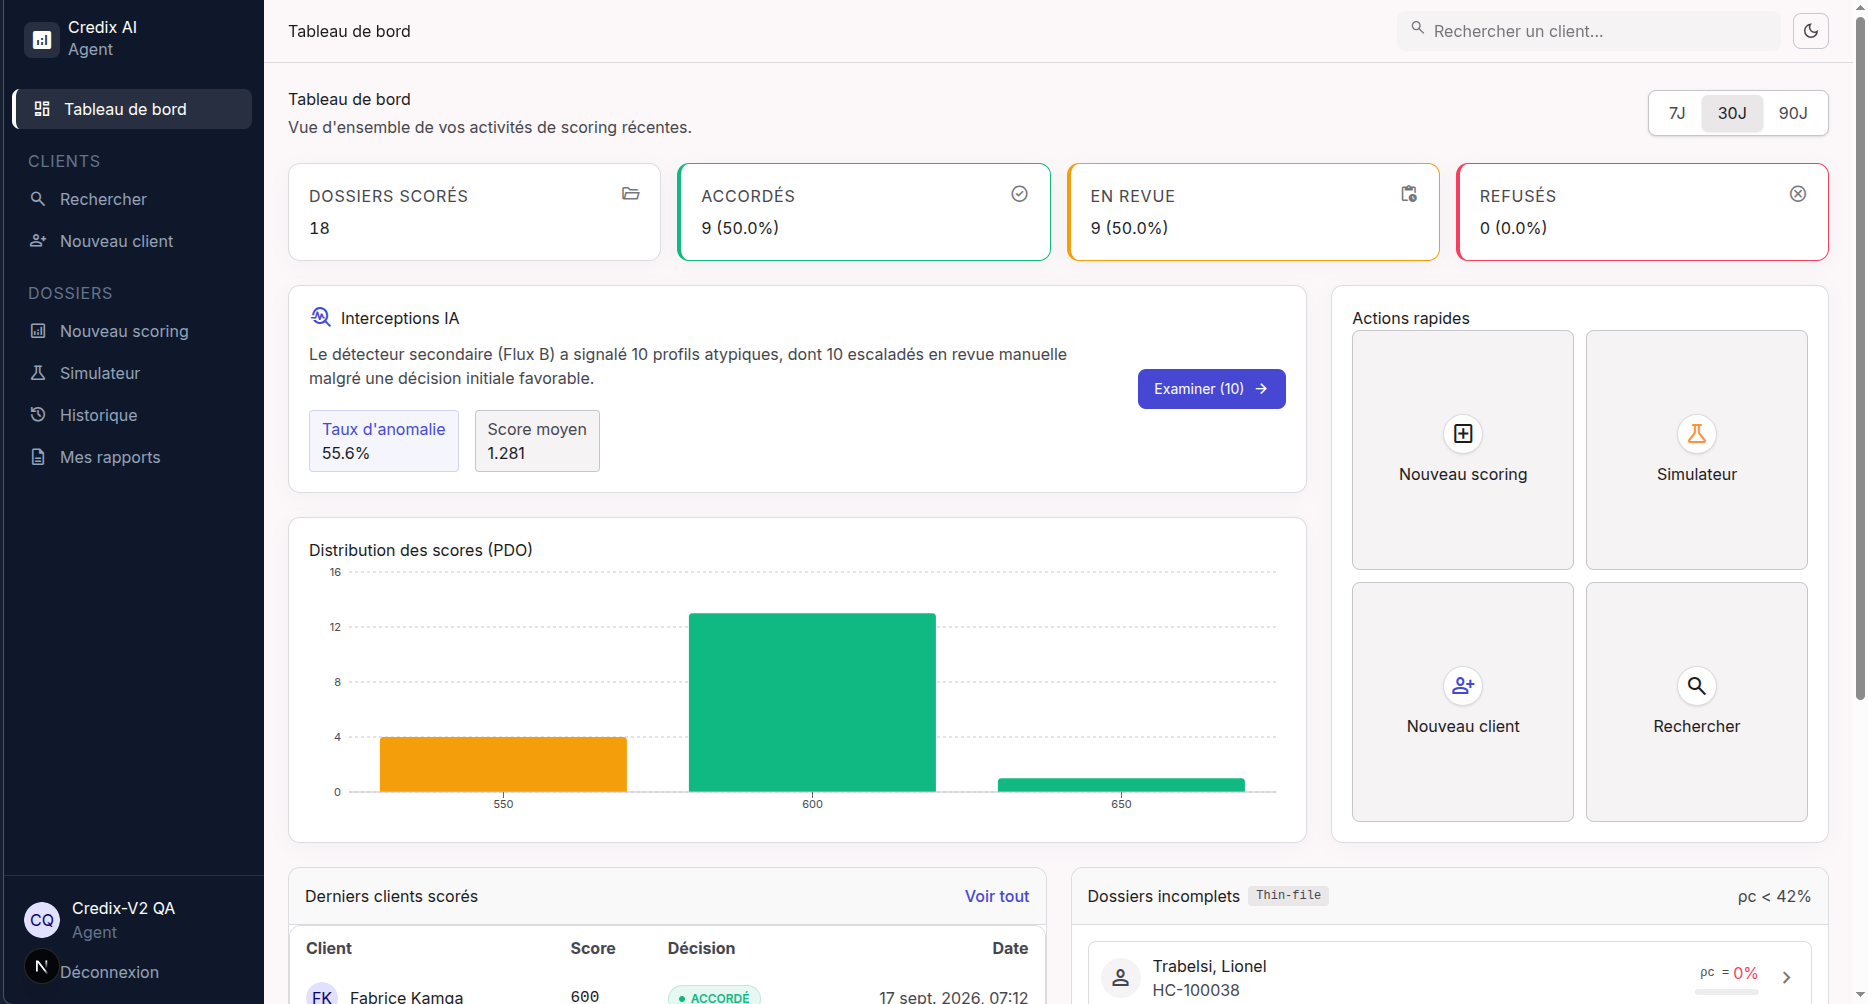
\includegraphics[width=\linewidth,height=0.75\textheight,keepaspectratio]{../images/readme/01_espace_agent.png}
  \caption{Espace Agent : tableau de bord.}
\end{figure}

\needspace{0.5\textheight}

\textbf{Page principale de l\textquotesingle espace Superviseur}

% --------------------------------------------------------------------
% CAPTURE : 02_espace_superviseur.png : Page principale de l'espace Superviseur (vue d'ensemble)
% Pour mettre votre image : changez seulement le nom du fichier dans \includegraphics{...}
\begin{figure}[H]
  \centering
  \def\CredixAlt{Page principale de l'espace Superviseur (vue d'ensemble)}%
  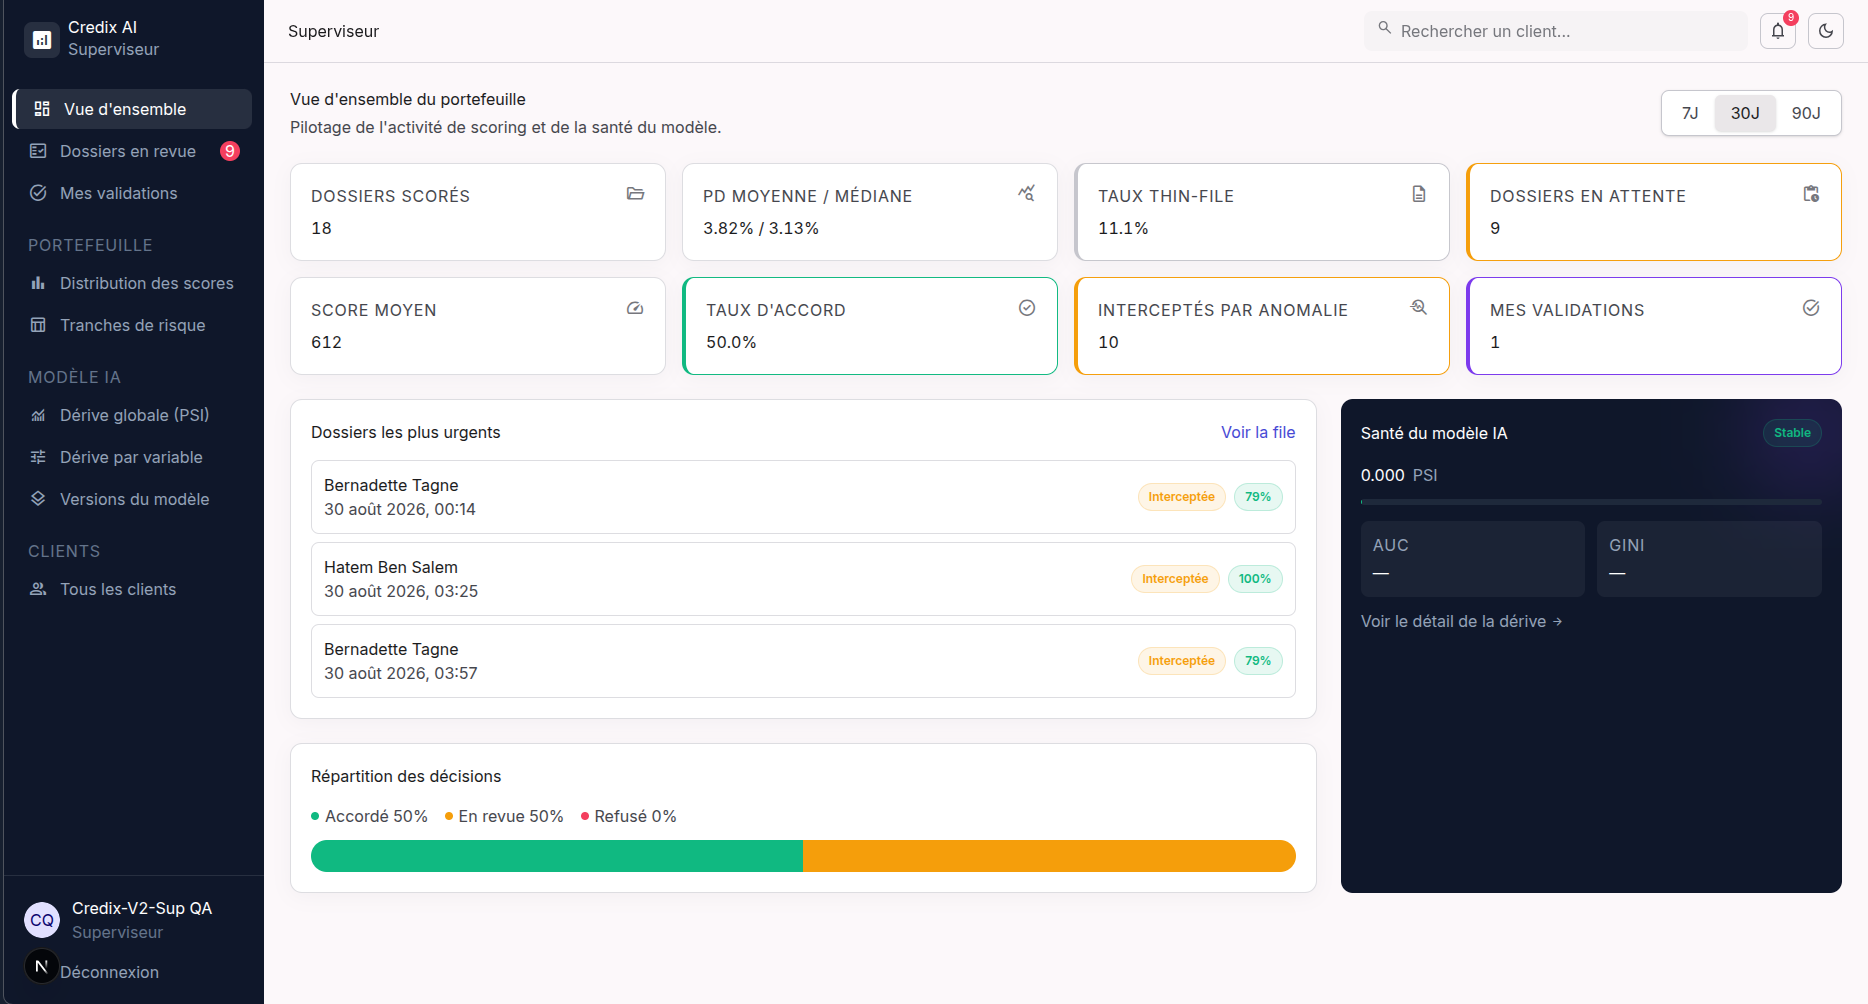
\includegraphics[width=\linewidth,height=0.75\textheight,keepaspectratio]{../images/readme/02_espace_superviseur.png}
  \caption{Espace Superviseur : vue d\textquotesingle ensemble.}
\end{figure}

\needspace{0.5\textheight}

\textbf{Page principale de l\textquotesingle espace Administrateur}

% --------------------------------------------------------------------
% CAPTURE : 03_espace_admin.png : Page principale de l'espace Administrateur (vue générale)
% Pour mettre votre image : changez seulement le nom du fichier dans \includegraphics{...}
\begin{figure}[H]
  \centering
  \def\CredixAlt{Page principale de l'espace Administrateur (vue générale)}%
  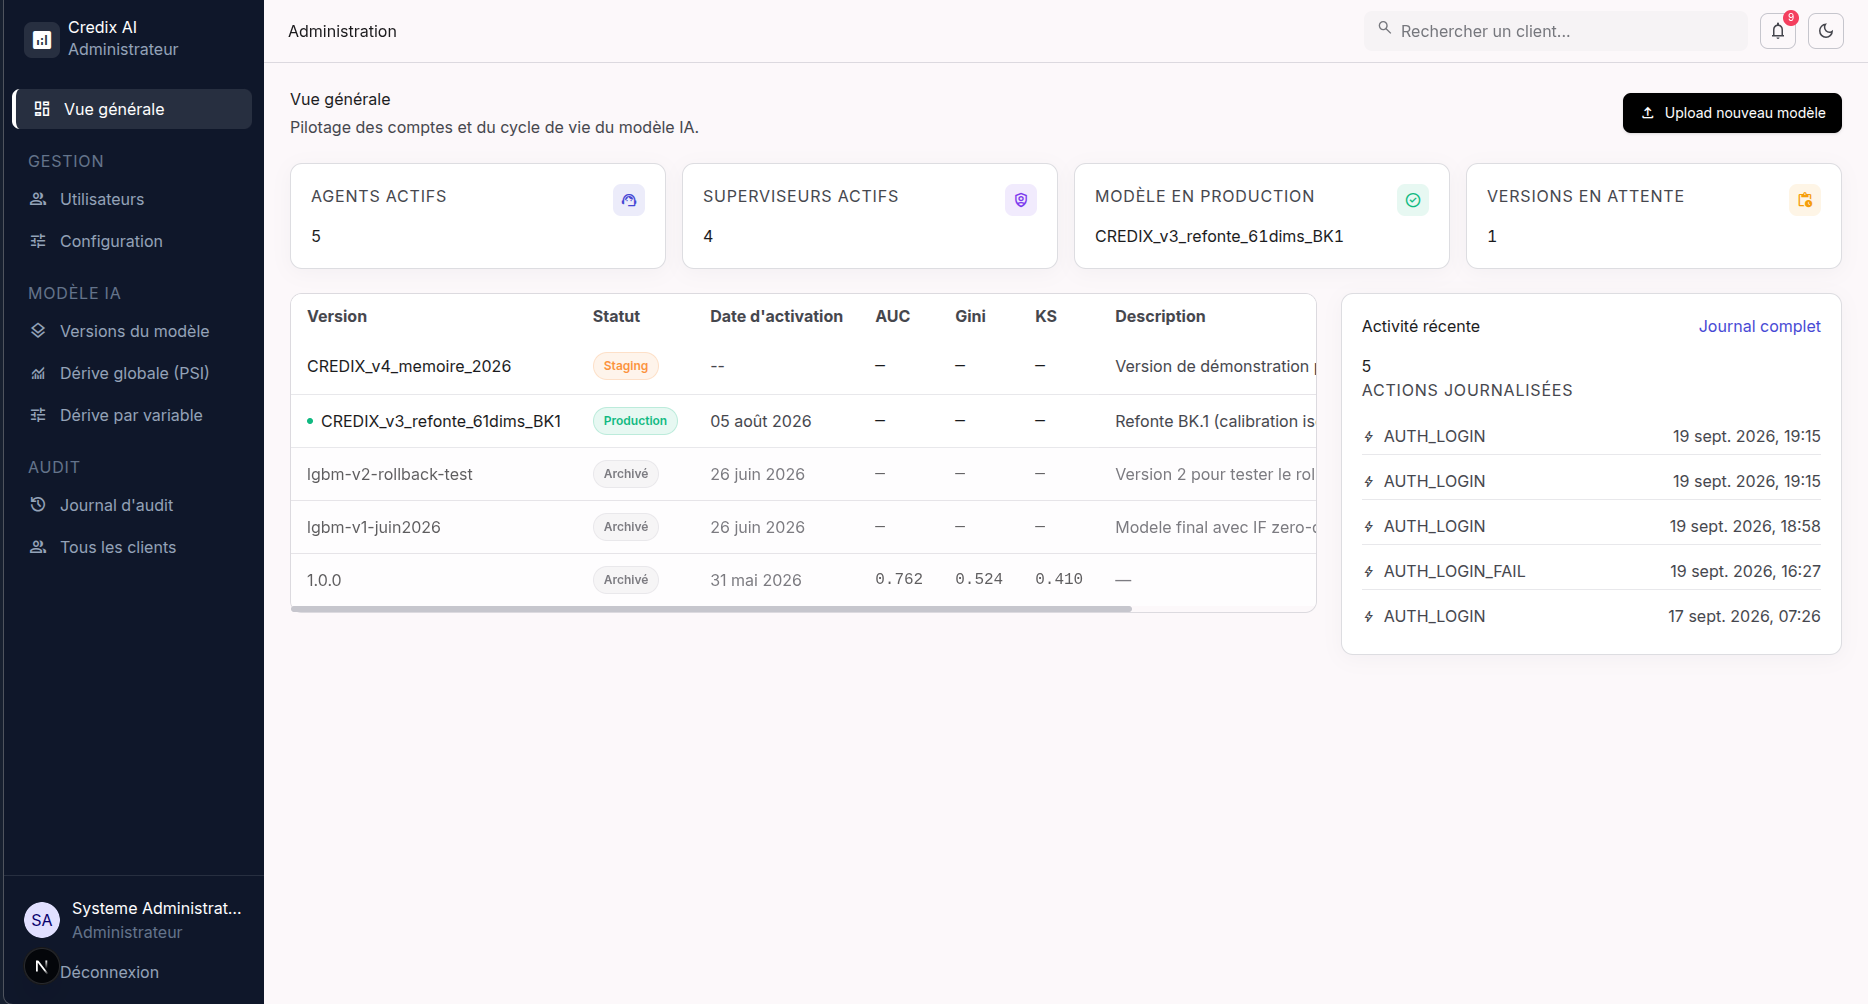
\includegraphics[width=\linewidth,height=0.75\textheight,keepaspectratio]{../images/readme/03_espace_admin.png}
  \caption{Espace Administrateur : vue générale.}
\end{figure}

La liste détaillée de tous les écrans se trouve dans
\texttt{credix-\allowbreak{}v2/\allowbreak{}FONCTIONNALITES.\allowbreak{}md}.

\subsubsection{1.5 Comment le système décide (les règles en
clair)}\label{15-comment-le-systuxe8me-duxe9cide-les-ruxe8gles-en-clair}

Le système travaille en \textbf{deux flux} qui se contrôlent
l\textquotesingle un l\textquotesingle autre :

\begin{itemize}
\tightlist
\item
  \textbf{Flux A (le score).} Un modèle (LightGBM) estime la probabilité
  de défaut (PD). Elle est corrigée par calibration, puis convertie en
  score : \texttt{Score\ =\ 515,06\ -\ 28,85\ x\ ln(PD\ /\ (1\ -\ PD))}.
\item
  \textbf{Flux B (le contrôle).} Un second modèle (un autoencodeur)
  mesure si le profil du client est \textbf{atypique}. Il ne juge pas le
  risque : il repère les dossiers sur lesquels le système ne devrait pas
  se prononcer seul.
\end{itemize}

\begin{longtable}[]{@{}
  >{\raggedright\arraybackslash}p{(\linewidth - 4\tabcolsep) * \real{0.2943}}
  >{\raggedright\arraybackslash}p{(\linewidth - 4\tabcolsep) * \real{0.2943}}
  >{\raggedright\arraybackslash}p{(\linewidth - 4\tabcolsep) * \real{0.3815}}@{}}
\toprule\noalign{}
\begin{minipage}[b]{\linewidth}\raggedright
Règle
\end{minipage} & \begin{minipage}[b]{\linewidth}\raggedright
Seuil
\end{minipage} & \begin{minipage}[b]{\linewidth}\raggedright
Conséquence
\end{minipage} \\
\midrule\noalign{}
\endhead
\bottomrule\noalign{}
\endlastfoot
PD inférieure à 10 \% (score au moins égal à 578,5) & Décision initiale
\textbf{ACCORDÉ} & Accord automatique \\
PD supérieure à 30 \% (score inférieur à 539,5) & Décision initiale
\textbf{REFUSÉ} & Refus automatique \\
PD entre les deux & Décision \textbf{REVUE MANUELLE} & Un superviseur
tranche \\
Profil atypique sur un dossier accordé & Seuil : percentile 95 (réglable
par l\textquotesingle administrateur) & Le dossier passe en
\textbf{revue manuelle}. Un dossier refusé, lui, reste refusé. \\
Couverture ρc inférieure à 0,42 & Information limitée & Bandeau «
confiance limitée » et recommandation de documents à demander au
client \\
Couverture ρc inférieure à 0,25 & Information très insuffisante &
\textbf{Revue manuelle forcée}, et le détecteur
d\textquotesingle anomalies est désactivé \\
\end{longtable}

Le \textbf{ρc n\textquotesingle est calculé qu\textquotesingle au moment
du scoring} : avant, un client affiche une couverture de 0,
c\textquotesingle est normal.

\subsubsection{1.6 Les outils utilisés}\label{16-les-outils-utilisuxe9s}

\begin{longtable}[]{@{}
  >{\raggedright\arraybackslash}p{(\linewidth - 2\tabcolsep) * \real{0.3946}}
  >{\raggedright\arraybackslash}p{(\linewidth - 2\tabcolsep) * \real{0.5754}}@{}}
\toprule\noalign{}
\begin{minipage}[b]{\linewidth}\raggedright
Domaine
\end{minipage} & \begin{minipage}[b]{\linewidth}\raggedright
Outils
\end{minipage} \\
\midrule\noalign{}
\endhead
\bottomrule\noalign{}
\endlastfoot
\textbf{Backend} (le « cerveau ») & Python 3.12, FastAPI 0.111, Uvicorn,
Pydantic 2 \\
\textbf{Modèle et calculs} & LightGBM 4.3, scikit-learn 1.6, optbinning
0.21 (transformation WoE), SHAP 0.45 (explications), TensorFlow CPU
(autoencodeur), pandas, NumPy \\
\textbf{Base de données} & MongoDB 7 (avec GridFS pour les fichiers du
modèle) \\
\textbf{Sécurité} & Jetons JWT, mots de passe hachés avec bcrypt \\
\textbf{Rapports PDF} & WeasyPrint, dans un petit service séparé \\
\textbf{Suivi des modèles} & MLflow 2.12 (démarré avec le reste ;
l\textquotesingle interface n\textquotesingle en dépend pas) \\
\textbf{Frontend} (l\textquotesingle interface web) & Next.js 15, React
19, TypeScript, Tailwind CSS 4, Radix UI, Recharts, react-hook-form et
zod, axios \\
\textbf{Lancement} & Docker et Docker Compose \\
\textbf{Conception} & Maquettes Google Stitch ; schémas draw.io et
PlantUML (dossier
\texttt{docs/\allowbreak{}diagrammes/\allowbreak{}}) \\
\textbf{Assistance à la conception et au développement} & Claude
(claude.ai en conversation, puis Claude Code dans VS Code). Le détail de
la méthode fait l\textquotesingle objet de guides séparés, dans
\texttt{docs/guides/}. \\
\end{longtable}

\begin{center}\rule{0.5\linewidth}{0.5pt}\end{center}

\subsection{2. Architecture : comment le projet est
organisé}\label{2-architecture--comment-le-projet-est-organisuxe9}

\subsubsection{2.1 Les cinq couches}\label{21-les-cinq-couches}

Le système est organisé en \textbf{cinq couches}, chacune avec une seule
responsabilité. Une couche ne dépend jamais d\textquotesingle une couche
au-dessus d\textquotesingle elle.

\begin{Verbatim}[breaklines=true,breakanywhere=true,fontsize=\footnotesize,frame=leftline,framerule=1.6pt,rulecolor=\color{credixblue},framesep=3mm,xleftmargin=2mm,xrightmargin=1mm]
        Navigateur web (l'utilisateur)
                    |
                    v
 [1] PRESENTATION         dossier credix-v2/                   port 3001
     affiche les écrans, recueille les saisies
                    |     requêtes HTTP avec un jeton JWT
                    v
 [2] INTERFACE            scoring-backend/app/routers/         port 8080
     APPLICATIVE          expose les opérations, vérifie l'identité et les droits
                    |
                    v
 [3] SERVICES DE          scoring-backend/app/services/
     DECISION             score, couverture rho_c, anomalie, règle finale, SHAP, PSI
              |                          |
              v                          v
 [4] MODELES              [5] PERSISTANCE
     scoring-backend/         MongoDB (port 27017)
     artefacts/               clients, demandes, décisions,
     (lecture seule)          journal d'audit, versions du modèle

 En plus :  service PDF (port 8001)   fabrique le compte rendu d'une décision
            MLflow (port 5000)        suivi des modèles
\end{Verbatim}

\subsubsection{2.2 Les services qui tournent, et leurs
ports}\label{22-les-services-qui-tournent-et-leurs-ports}

\begin{longtable}[]{@{}
  >{\raggedright\arraybackslash}p{(\linewidth - 4\tabcolsep) * \real{0.2387}}
  >{\raggedright\arraybackslash}p{(\linewidth - 4\tabcolsep) * \real{0.1925}}
  >{\raggedright\arraybackslash}p{(\linewidth - 4\tabcolsep) * \real{0.5389}}@{}}
\toprule\noalign{}
\begin{minipage}[b]{\linewidth}\raggedright
Service
\end{minipage} & \begin{minipage}[b]{\linewidth}\raggedright
Rôle
\end{minipage} & \begin{minipage}[b]{\linewidth}\raggedright
Adresse sur votre ordinateur
\end{minipage} \\
\midrule\noalign{}
\endhead
\bottomrule\noalign{}
\endlastfoot
Frontend (Next.js) & L\textquotesingle interface web &
\url{http://localhost:3001} \\
API (FastAPI), service \texttt{api} & Le backend &
\url{http://localhost:8080} (documentation interactive :
\url{http://localhost:8080/docs}) \\
MongoDB, service \texttt{mongodb} & La base de données &
\texttt{localhost:27017} \\
Service PDF, service \texttt{pdf-worker} & Fabrique les rapports PDF &
\url{http://localhost:8001} \\
MLflow, service \texttt{mlflow} & Suivi des modèles &
\url{http://localhost:5000} \\
\end{longtable}

Le backend et ses trois services annexes tournent dans des
\textbf{conteneurs Docker}. Le frontend tourne directement sur votre
machine, avec Node.js.

\subsubsection{2.3 L\textquotesingle arborescence des
dossiers}\label{23-larborescence-des-dossiers}

\begin{Verbatim}[breaklines=true,breakanywhere=true,fontsize=\footnotesize,frame=leftline,framerule=1.6pt,rulecolor=\color{credixblue},framesep=3mm,xleftmargin=2mm,xrightmargin=1mm]
credix/                          dossier créé par « git clone »
|-- README.md                    ce document
|-- scoring-backend/             LE BACKEND
|   |-- app/                     le code de l'API
|   |   |-- main.py              démarrage, chargement du modèle, route /health
|   |   |-- routers/             les routes : auth, scoring, clients, decisions,
|   |   |                        dashboard, monitoring, admin, upload_model
|   |   |-- services/            la logique de décision : pipeline (WoE et LightGBM),
|   |   |                        calibration, score PDO, couverture rho_c, SHAP, PSI,
|   |   |                        percentiles, client du service PDF
|   |   |-- schemas/             la forme des données échangées
|   |   |-- core/                configuration (config.py) et sécurité (JWT, droits)
|   |   `-- db/                  accès à MongoDB et à GridFS
|   |-- artefacts/               les 16 fichiers du modèle entraîné (3,5 Mo),
|   |                            dont 14 chargés par l'API au démarrage
|   |-- demo_data/               phrases d'explication et clients de démonstration
|   |-- scripts/                 scripts de premier lancement (voir section 5)
|   |-- adapters/, configs/      lecture des données Home Credit (rechargement complet)
|   |-- pdf-worker/              le petit service qui fabrique les PDF
|   |-- mock/, tests/            fichiers factices et tests
|   |-- contexte claude code/    notes de travail avec Claude Code
|   |-- docker-compose.yml       la description des 4 conteneurs
|   |-- Dockerfile.api           la recette de fabrication de l'image de l'API
|   |-- requirements.txt         les bibliothèques Python
|   |-- .env.example             le modèle du fichier de configuration
|   `-- README.md                documentation technique détaillée du backend
|-- credix-v2/                   LE FRONTEND
|   |-- app/                     les pages (un dossier par écran)
|   |-- components/              les briques visuelles réutilisables
|   |-- contexts/, hooks/, lib/  connexion, appels à l'API, types
|   |-- package.json             les bibliothèques JavaScript et les commandes npm
|   |-- .env.example             le modèle du fichier de configuration
|   `-- FONCTIONNALITES.md       la liste détaillée des écrans
|-- docs/                        schémas (diagrammes/), captures (captures_memoire/),
|                                images (images/), guides (guides/), PDF (pdf/),
|                                fichiers LaTeX (tex/), outils de fabrication (build/)
`-- stitch_credix_design_system/ cahier des charges du frontend et système de design
\end{Verbatim}

\begin{center}\rule{0.5\linewidth}{0.5pt}\end{center}

\subsection{3. Ce qu\textquotesingle il faut installer avant de
commencer}\label{3-ce-quil-faut-installer-avant-de-commencer}

\subsubsection{3.1 Ordinateur
nécessaire}\label{31-ordinateur-nuxe9cessaire}

\begin{longtable}[]{@{}
  >{\raggedright\arraybackslash}p{(\linewidth - 2\tabcolsep) * \real{0.2071}}
  >{\raggedright\arraybackslash}p{(\linewidth - 2\tabcolsep) * \real{0.7629}}@{}}
\toprule\noalign{}
\begin{minipage}[b]{\linewidth}\raggedright
Ressource
\end{minipage} & \begin{minipage}[b]{\linewidth}\raggedright
Minimum conseillé
\end{minipage} \\
\midrule\noalign{}
\endhead
\bottomrule\noalign{}
\endlastfoot
Système & Linux 64 bits (testé sur Ubuntu) \\
Espace disque libre & 10 Go (les images Docker pèsent environ 6 Go) \\
Mémoire vive (RAM) & 8 Go recommandés \\
Ports libres & 3001, 8080, 8001, 5000, 27017 \\
Connexion Internet & Oui, pour le premier lancement (téléchargement des
images et des bibliothèques) \\
\end{longtable}

\subsubsection{3.2 Les outils}\label{32-les-outils}

\begin{longtable}[]{@{}
  >{\raggedright\arraybackslash}p{(\linewidth - 4\tabcolsep) * \real{0.1712}}
  >{\raggedright\arraybackslash}p{(\linewidth - 4\tabcolsep) * \real{0.4993}}
  >{\raggedright\arraybackslash}p{(\linewidth - 4\tabcolsep) * \real{0.2996}}@{}}
\toprule\noalign{}
\begin{minipage}[b]{\linewidth}\raggedright
Outil
\end{minipage} & \begin{minipage}[b]{\linewidth}\raggedright
À quoi il sert
\end{minipage} & \begin{minipage}[b]{\linewidth}\raggedright
Version utilisée pour les tests
\end{minipage} \\
\midrule\noalign{}
\endhead
\bottomrule\noalign{}
\endlastfoot
\textbf{Git} & Récupérer et versionner le projet & 2.43 \\
\textbf{Docker} et \textbf{Docker Compose} & Lancer le backend, la base
de données et les services annexes sans les installer un par un & Docker
29.5, Compose 5.1 \\
\textbf{Node.js} et \textbf{npm} & Lancer et compiler le frontend & Node
22.22, npm 11.14 (Node 18.18 minimum) \\
\textbf{curl} & Vérifier depuis le terminal que les services répondent &
8.16 \\
\textbf{OpenSSL} & Fabriquer une clé secrète aléatoire & 3.5 \\
\end{longtable}

\subsubsection{3.3 Vérifier ce qui est déjà
installé}\label{33-vuxe9rifier-ce-qui-est-duxe9juxe0-installuxe9}

Ouvrez un terminal et tapez ces commandes, une par une :

\begin{Verbatim}[breaklines=true,breakanywhere=true,fontsize=\footnotesize,frame=leftline,framerule=1.6pt,rulecolor=\color{credixblue},framesep=3mm,xleftmargin=2mm,xrightmargin=1mm]
git --version
docker --version
docker compose version
node --version
npm --version
curl --version
openssl version
\end{Verbatim}

\textbf{Ce que fait chaque commande :} elle affiche le numéro de version
de l\textquotesingle outil.

\textbf{Résultat attendu (les numéros peuvent différer légèrement) :}

\begin{Verbatim}[breaklines=true,breakanywhere=true,fontsize=\footnotesize,frame=leftline,framerule=1.6pt,rulecolor=\color{credixblue},framesep=3mm,xleftmargin=2mm,xrightmargin=1mm]
git version 2.43.0
Docker version 29.5.3, build d1c06ef
Docker Compose version v5.1.4
v22.22.0
11.14.1
curl 8.16.0 (Linux) libcurl/8.16.0 ...
OpenSSL 3.5.5 27 Jan 2026 ...
\end{Verbatim}

\textbf{Si une commande répond « command not found » :}
l\textquotesingle outil n\textquotesingle est pas installé, passez à la
section 3.4 pour cet outil.

\subsubsection{3.4 Installer ce qui manque (Ubuntu ou
Debian)}\label{34-installer-ce-qui-manque-ubuntu-ou-debian}

\begin{quote}
Les commandes de cette section viennent de la documentation officielle
de chaque outil. Elles n\textquotesingle ont \textbf{pas été rejouées}
pour ce guide, car la machine de test avait déjà tout installé. En cas
de doute, suivez la documentation officielle indiquée.
\end{quote}

\textbf{Git, curl et OpenSSL :}

\begin{Verbatim}[breaklines=true,breakanywhere=true,fontsize=\footnotesize,frame=leftline,framerule=1.6pt,rulecolor=\color{credixblue},framesep=3mm,xleftmargin=2mm,xrightmargin=1mm]
sudo apt-get update
sudo apt-get install -y git curl openssl
\end{Verbatim}

\textbf{Docker et Docker Compose} (documentation officielle :
\url{https://docs.docker.com/engine/install/ubuntu/}) :

\begin{Verbatim}[breaklines=true,breakanywhere=true,fontsize=\footnotesize,frame=leftline,framerule=1.6pt,rulecolor=\color{credixblue},framesep=3mm,xleftmargin=2mm,xrightmargin=1mm]
sudo apt-get update
sudo apt-get install -y ca-certificates curl
sudo install -m 0755 -d /etc/apt/keyrings
sudo curl -fsSL https://download.docker.com/linux/ubuntu/gpg -o /etc/apt/keyrings/docker.asc
sudo chmod a+r /etc/apt/keyrings/docker.asc
echo "deb [arch=$(dpkg --print-architecture) signed-by=/etc/apt/keyrings/docker.asc] https://download.docker.com/linux/ubuntu $(. /etc/os-release && echo "${UBUNTU_CODENAME:-$VERSION_CODENAME}") stable" | sudo tee /etc/apt/sources.list.d/docker.list > /dev/null
sudo apt-get update
sudo apt-get install -y docker-ce docker-ce-cli containerd.io docker-buildx-plugin docker-compose-plugin
\end{Verbatim}

Ensuite, \textbf{autorisez votre utilisateur à utiliser Docker sans
\texttt{sudo}} (sinon vous aurez l\textquotesingle erreur « permission
denied ») :

\begin{Verbatim}[breaklines=true,breakanywhere=true,fontsize=\footnotesize,frame=leftline,framerule=1.6pt,rulecolor=\color{credixblue},framesep=3mm,xleftmargin=2mm,xrightmargin=1mm]
sudo usermod -aG docker $USER
\end{Verbatim}

\textbf{Fermez votre session Linux puis rouvrez-la} (ou redémarrez),
puis testez :

\begin{Verbatim}[breaklines=true,breakanywhere=true,fontsize=\footnotesize,frame=leftline,framerule=1.6pt,rulecolor=\color{credixblue},framesep=3mm,xleftmargin=2mm,xrightmargin=1mm]
docker run --rm hello-world
\end{Verbatim}

\textbf{Résultat attendu :} un message qui contient
\texttt{Hello\ from\ Docker!}.

\textbf{Node.js et npm} (avec l\textquotesingle outil nvm, documentation
: \url{https://github.com/nvm-sh/nvm}) :

\begin{Verbatim}[breaklines=true,breakanywhere=true,fontsize=\footnotesize,frame=leftline,framerule=1.6pt,rulecolor=\color{credixblue},framesep=3mm,xleftmargin=2mm,xrightmargin=1mm]
curl -o- https://raw.githubusercontent.com/nvm-sh/nvm/v0.40.3/install.sh | bash
\end{Verbatim}

Fermez puis rouvrez le terminal, et tapez :

\begin{Verbatim}[breaklines=true,breakanywhere=true,fontsize=\footnotesize,frame=leftline,framerule=1.6pt,rulecolor=\color{credixblue},framesep=3mm,xleftmargin=2mm,xrightmargin=1mm]
nvm install 22
node --version
\end{Verbatim}

\textbf{Résultat attendu :} \texttt{v22.} suivi de deux numéros.

\begin{center}\rule{0.5\linewidth}{0.5pt}\end{center}

\subsection{4. Récupérer le projet depuis
GitHub}\label{4-ruxe9cupuxe9rer-le-projet-depuis-github}

\subsubsection{4.1 Le lien du dépôt}\label{41-le-lien-du-duxe9puxf4t}

\begin{itemize}
\tightlist
\item
  Page du projet : \url{https://github.com/HendrixPenka2/credix}
\item
  Adresse à utiliser pour copier le projet (HTTPS) :
  \texttt{https:/\allowbreak{}/\allowbreak{}github.\allowbreak{}com/\allowbreak{}HendrixPenka2/\allowbreak{}credix.\allowbreak{}git}
\end{itemize}

Le dépôt est \textbf{privé} : seules les personnes invitées peuvent le
voir et le copier. Avant de faire \texttt{git\ clone}, il faut donc :

\begin{enumerate}
\def\labelenumi{\arabic{enumi}.}
\tightlist
\item
  \textbf{avoir un compte GitHub} (gratuit) ;
\item
  \textbf{être invité par l\textquotesingle auteur} comme collaborateur
  (l\textquotesingle auteur ouvre le dépôt sur GitHub, puis
  \emph{Settings}, \emph{Collaborators}, \emph{Add people}) ; vous
  recevez un e-mail d\textquotesingle invitation, à \textbf{accepter} ;
\item
  \textbf{créer un jeton d\textquotesingle accès personnel}, car Git
  n\textquotesingle accepte plus le mot de passe du compte : sur GitHub,
  menu de votre photo de profil, \emph{Settings}, \emph{Developer
  settings}, \emph{Personal access tokens}, \emph{Tokens (classic)},
  \emph{Generate new token}, puis \emph{Generate new token (classic)} ;
  donnez-lui un nom, cochez la permission \textbf{\texttt{repo}},
  cliquez sur \emph{Generate token}, puis \textbf{copiez le jeton
  affiché} (il n\textquotesingle est montré qu\textquotesingle une seule
  fois). Documentation :
  \url{https://docs.github.com/fr/authentication}.
\end{enumerate}

\begin{quote}
Ces trois étapes exigent un compte GitHub et n\textquotesingle ont pas
pu être rejouées pour ce guide.
\end{quote}

\subsubsection{4.2 Copier le projet sur votre
ordinateur}\label{42-copier-le-projet-sur-votre-ordinateur}

\begin{Verbatim}[breaklines=true,breakanywhere=true,fontsize=\footnotesize,frame=leftline,framerule=1.6pt,rulecolor=\color{credixblue},framesep=3mm,xleftmargin=2mm,xrightmargin=1mm]
cd ~
git clone https://github.com/HendrixPenka2/credix.git
cd credix
ls
\end{Verbatim}

\textbf{Ce que fait chaque commande :}

\begin{longtable}[]{@{}
  >{\raggedright\arraybackslash}p{(\linewidth - 2\tabcolsep) * \real{0.2071}}
  >{\raggedright\arraybackslash}p{(\linewidth - 2\tabcolsep) * \real{0.7629}}@{}}
\toprule\noalign{}
\begin{minipage}[b]{\linewidth}\raggedright
Commande
\end{minipage} & \begin{minipage}[b]{\linewidth}\raggedright
Effet
\end{minipage} \\
\midrule\noalign{}
\endhead
\bottomrule\noalign{}
\endlastfoot
\texttt{cd\ \textasciitilde{}} & Va dans votre dossier personnel \\
\texttt{git\ clone\ \textless{}adresse\textgreater{}} & \textbf{Copie
tout le projet} (le code et son historique) dans un nouveau dossier
\texttt{credix} \\
\texttt{cd\ credix} & Entre dans ce dossier \\
\texttt{ls} & Liste son contenu \\
\end{longtable}

\textbf{Pendant le \texttt{git\ clone}, Git vous demande de vous
identifier} (le dépôt est privé) :

\begin{Verbatim}[breaklines=true,breakanywhere=true,fontsize=\footnotesize,frame=leftline,framerule=1.6pt,rulecolor=\color{credixblue},framesep=3mm,xleftmargin=2mm,xrightmargin=1mm]
Username for 'https://github.com':
Password for 'https://votre_nom@github.com':
\end{Verbatim}

Tapez votre \textbf{nom d\textquotesingle utilisateur GitHub}, puis, à
la ligne « Password », \textbf{collez le jeton} créé en 4.1 (rien ne
s\textquotesingle affiche pendant la saisie, c\textquotesingle est
normal), puis appuyez sur \texttt{Entrée}. Pour ne pas le retaper à
chaque fois, vous pouvez taper une fois
\texttt{git\ config\ -\/-global\ credential.helper\ store} avant le
clone (attention : le jeton est alors enregistré en clair dans votre
dossier personnel).

\textbf{Si vous obtenez \texttt{Repository\ not\ found} ou
\texttt{Authentication\ failed} :} l\textquotesingle invitation
n\textquotesingle a pas été acceptée, ou vous avez saisi le mot de passe
du compte au lieu du jeton.

\textbf{Résultat attendu de \texttt{ls} :}

\begin{Verbatim}[breaklines=true,breakanywhere=true,fontsize=\footnotesize,frame=leftline,framerule=1.6pt,rulecolor=\color{credixblue},framesep=3mm,xleftmargin=2mm,xrightmargin=1mm]
credix-v2  docs  README.md  scoring-backend  stitch_credix_design_system
\end{Verbatim}

\subsubsection{4.3 Vérifier la copie}\label{43-vuxe9rifier-la-copie}

\begin{Verbatim}[breaklines=true,breakanywhere=true,fontsize=\footnotesize,frame=leftline,framerule=1.6pt,rulecolor=\color{credixblue},framesep=3mm,xleftmargin=2mm,xrightmargin=1mm]
git status
git log --oneline -3
ls scoring-backend/artefacts | wc -l
\end{Verbatim}

\textbf{Ce que fait chaque commande :} \texttt{git\ status} indique la
branche et si des fichiers ont changé ;
\texttt{git\ log\ -\/-oneline\ -3} affiche les 3 dernières modifications
enregistrées ; la dernière commande \textbf{compte les fichiers du
modèle}.

\textbf{Résultat attendu :} \texttt{git\ status} indique « Sur la
branche main » et « la copie de travail est propre » ; la dernière
commande affiche \textbf{\texttt{16}}.

\textbf{Si vous obtenez un autre nombre que 16 :} la copie est
incomplète. Supprimez le dossier \texttt{credix}
(\texttt{cd\ \textasciitilde{}\ \&\&\ rm\ -rf\ credix}) et recommencez
le \texttt{git\ clone}.

\begin{center}\rule{0.5\linewidth}{0.5pt}\end{center}

\subsection{5. Lancer le backend}\label{5-lancer-le-backend}

Toutes les commandes de cette section se tapent \textbf{dans le dossier
\texttt{scoring-\allowbreak{}backend}}. Placez-vous-y :

\begin{Verbatim}[breaklines=true,breakanywhere=true,fontsize=\footnotesize,frame=leftline,framerule=1.6pt,rulecolor=\color{credixblue},framesep=3mm,xleftmargin=2mm,xrightmargin=1mm]
cd ~/credix/scoring-backend
pwd
\end{Verbatim}

\textbf{Résultat attendu de \texttt{pwd} (affiche le dossier courant) :}
\texttt{/\allowbreak{}home/\allowbreak{}votre\_\allowbreak{}nom/\allowbreak{}credix/\allowbreak{}scoring-\allowbreak{}backend}.

\subsubsection{\texorpdfstring{5.1 Configurer : créer le fichier
\texttt{.env}}{5.1 Configurer : créer le fichier .env}}\label{51-configurer--cruxe9er-le-fichier-env}

Le fichier \texttt{.env} contient les réglages du backend, dont un
\textbf{secret} qui ne doit jamais être publié. Le dépôt ne contient
qu\textquotesingle un modèle, \texttt{.env.example}.

\begin{Verbatim}[breaklines=true,breakanywhere=true,fontsize=\footnotesize,frame=leftline,framerule=1.6pt,rulecolor=\color{credixblue},framesep=3mm,xleftmargin=2mm,xrightmargin=1mm]
cp .env.example .env
sed -i "s|^JWT_SECRET=.*|JWT_SECRET=$(openssl rand -hex 32)|" .env
grep -E "^(USE_MOCK_ARTEFACTS|MONGO_URI|ALLOWED_ORIGINS|JWT_SECRET)=" .env
\end{Verbatim}

\textbf{Ce que fait chaque commande :}

\begin{longtable}[]{@{}
  >{\raggedright\arraybackslash}p{(\linewidth - 2\tabcolsep) * \real{0.2477}}
  >{\raggedright\arraybackslash}p{(\linewidth - 2\tabcolsep) * \real{0.7223}}@{}}
\toprule\noalign{}
\begin{minipage}[b]{\linewidth}\raggedright
Commande
\end{minipage} & \begin{minipage}[b]{\linewidth}\raggedright
Effet
\end{minipage} \\
\midrule\noalign{}
\endhead
\bottomrule\noalign{}
\endlastfoot
\texttt{cp\ .env.example\ .env} & Copie le modèle vers le vrai fichier
de configuration \\
\texttt{sed\ -i\ "s\textbar{}...\textbar{}...\textbar{}"\ .env} &
Remplace la ligne \texttt{JWT\_SECRET=} par \textbf{une clé secrète
aléatoire de 64 caractères}, fabriquée par
\texttt{openssl\ rand\ -hex\ 32}. Cette clé sert à signer les jetons de
connexion. \\
\texttt{grep\ -E\ ...\ .env} & Affiche les 4 réglages les plus
importants pour que vous les contrôliez \\
\end{longtable}

\textbf{Résultat attendu (la valeur de \texttt{JWT\_SECRET} sera
différente chez vous, mais elle doit faire 64 caractères) :}

\begin{Verbatim}[breaklines=true,breakanywhere=true,fontsize=\footnotesize,frame=leftline,framerule=1.6pt,rulecolor=\color{credixblue},framesep=3mm,xleftmargin=2mm,xrightmargin=1mm]
USE_MOCK_ARTEFACTS=false
MONGO_URI=mongodb://mongodb:27017
JWT_SECRET=3f9c1e...(64 caractères au total)
ALLOWED_ORIGINS=http://localhost:3000,http://localhost:3001,http://localhost:5173
\end{Verbatim}

\textbf{Ce que signifient ces réglages :}

\begin{itemize}
\tightlist
\item
  \texttt{USE\_\allowbreak{}MOCK\_\allowbreak{}ARTEFACTS=false} : on
  utilise le \textbf{vrai modèle} (le dossier \texttt{artefacts/}) et
  non des fichiers factices.
\item
  \texttt{MONGO\_\allowbreak{}URI=mongodb:/\allowbreak{}/\allowbreak{}mongodb:27017}
  : l\textquotesingle adresse de la base de données \textbf{à
  l\textquotesingle intérieur de Docker} ; ne la changez pas.
\item
  \texttt{ALLOWED\_\allowbreak{}ORIGINS} : les adresses autorisées à
  appeler l\textquotesingle API.
  \textbf{\texttt{http:/\allowbreak{}/\allowbreak{}localhost:3001} doit
  y figurer}, sinon le navigateur bloquera le frontend.
\item
  Les autres lignes du fichier (\texttt{GOOGLE\_API\_KEY},
  \texttt{HOME\_\allowbreak{}CREDIT\_\allowbreak{}DATA\_\allowbreak{}DIR}\ldots)
  sont \textbf{facultatives} et ne servent pas pour tester ; le fichier
  \texttt{.env.example} les explique une par une.
\end{itemize}

\textbf{Si \texttt{JWT\_SECRET} contient encore \texttt{CHANGE\_MOI} :}
la deuxième commande a échoué ; vérifiez qu\textquotesingle OpenSSL est
installé (\texttt{openssl\ version}) et relancez-la.

\subsubsection{5.2 Démarrer les
conteneurs}\label{52-duxe9marrer-les-conteneurs}

\begin{Verbatim}[breaklines=true,breakanywhere=true,fontsize=\footnotesize,frame=leftline,framerule=1.6pt,rulecolor=\color{credixblue},framesep=3mm,xleftmargin=2mm,xrightmargin=1mm]
docker compose up -d --build
\end{Verbatim}

\textbf{Ce que fait cette commande :}

\begin{itemize}
\tightlist
\item
  \texttt{docker\ compose} lit le fichier
  \texttt{docker-\allowbreak{}compose.\allowbreak{}yml}, qui décrit
  \textbf{4 conteneurs} : l\textquotesingle API, MongoDB, MLflow et le
  service PDF ;
\item
  \texttt{up} les \textbf{démarre} ;
\item
  \texttt{-d} les lance \textbf{en arrière-plan} (vous récupérez la main
  dans le terminal) ;
\item
  \texttt{-\/-build} \textbf{fabrique d\textquotesingle abord les
  images} qui en ont besoin (l\textquotesingle API et le service PDF).
\end{itemize}

\textbf{Ce qu\textquotesingle il faut savoir :} au \textbf{premier
lancement}, Docker télécharge des images (MongoDB, MLflow) et
\textbf{fabrique celles de l\textquotesingle API et du service PDF} : il
installe des paquets système puis des bibliothèques Python, dont
TensorFlow (250 Mo à lui seul). Il y a \textbf{environ 700 Mo à
télécharger}, donc la durée dépend surtout de votre connexion. Lors de
notre test, avec une connexion lente (de 75 à 300 Ko/s), cela a duré
\textbf{environ 50 minutes} (dont 45 pour l\textquotesingle installation
des bibliothèques Python de l\textquotesingle API) ; avec une bonne
connexion, comptez nettement moins. Prévoyez aussi \textbf{de la place
sur le disque} : la construction a besoin d\textquotesingle environ 4 Go
de marge temporaire à la toute fin (voir la section 3.1). Les lancements
suivants sont rapides : environ \textbf{une minute} (les images sont
déjà fabriquées).

\textbf{Comment savoir que c\textquotesingle est terminé ?}

\begin{itemize}
\tightlist
\item
  La commande affiche beaucoup de lignes
  (\texttt{\#15\ {[}api\ ...{]}\ Downloading\ ...}) et \textbf{ne vous
  rend pas la main} tant qu\textquotesingle elle travaille :
  l\textquotesingle invite du terminal (le \texttt{\$}) ne réapparaît
  pas.
\item
  Pendant le téléchargement d\textquotesingle un gros fichier comme
  TensorFlow, \textbf{rien ne s\textquotesingle affiche pendant
  plusieurs minutes} : ce n\textquotesingle est pas un blocage. Pour le
  vérifier, ouvrez un \textbf{autre terminal} et tapez
  \texttt{docker\ ps} : tant que vos conteneurs \texttt{scoring-...}
  n\textquotesingle apparaissent pas dans la liste, la construction est
  en cours.
\item
  C\textquotesingle est \textbf{terminé} quand l\textquotesingle invite
  du terminal \textbf{réapparaît}, après les lignes
  \texttt{Container\ ...\ Started} ci-dessous. Passez alors à la section
  5.3.
\end{itemize}

\textbf{Résultat attendu à la fin :} des lignes de ce type (le mot «
error » ne doit pas apparaître) :

\begin{Verbatim}[breaklines=true,breakanywhere=true,fontsize=\footnotesize,frame=leftline,framerule=1.6pt,rulecolor=\color{credixblue},framesep=3mm,xleftmargin=2mm,xrightmargin=1mm]
 Container scoring-mongodb Started
 Container scoring-mlflow Started
 Container scoring-pdf Started
 Container scoring-api Started
\end{Verbatim}

\subsubsection{5.3 Vérifier que le backend
tourne}\label{53-vuxe9rifier-que-le-backend-tourne}

Le démarrage de l\textquotesingle API prend \textbf{une à deux minutes}
(elle charge le modèle en mémoire). Faites les vérifications dans cet
ordre.

\paragraph{Vérification 1 : l\textquotesingle état des
conteneurs}\label{vuxe9rification-1--luxe9tat-des-conteneurs}

\begin{Verbatim}[breaklines=true,breakanywhere=true,fontsize=\footnotesize,frame=leftline,framerule=1.6pt,rulecolor=\color{credixblue},framesep=3mm,xleftmargin=2mm,xrightmargin=1mm]
docker compose ps
\end{Verbatim}

\textbf{Ce que fait la commande :} elle liste les conteneurs du projet
et leur état.

\textbf{Résultat attendu :}

\begin{Verbatim}[breaklines=true,breakanywhere=true,fontsize=\footnotesize,frame=leftline,framerule=1.6pt,rulecolor=\color{credixblue},framesep=3mm,xleftmargin=2mm,xrightmargin=1mm]
NAME              IMAGE                           COMMAND                  SERVICE      CREATED         STATUS                   PORTS
scoring-api       scoring-backend-api             "uvicorn app.main:ap…"   api          2 minutes ago   Up 2 minutes (healthy)   0.0.0.0:8080->8000/tcp, [::]:8080->8000/tcp
scoring-mlflow    ghcr.io/mlflow/mlflow:v2.12.1   "mlflow server --hos…"   mlflow       2 minutes ago   Up 2 minutes             0.0.0.0:5000->5000/tcp, [::]:5000->5000/tcp
scoring-mongodb   mongo:7.0                       "docker-entrypoint.s…"   mongodb      2 minutes ago   Up 2 minutes (healthy)   0.0.0.0:27017->27017/tcp, [::]:27017->27017/tcp
scoring-pdf       scoring-backend-pdf-worker      "uvicorn main:app --…"   pdf-worker   2 minutes ago   Up 2 minutes             0.0.0.0:8001->8001/tcp, [::]:8001->8001/tcp
\end{Verbatim}

\textbf{Comment lire ce tableau :} les \textbf{4 conteneurs} doivent
être \texttt{Up}. \texttt{scoring-api} et
\texttt{scoring-\allowbreak{}mongodb} doivent afficher
\textbf{\texttt{(healthy)}}. Juste après le démarrage,
\texttt{scoring-api} peut afficher \texttt{(health:\ starting)} :
\textbf{attendez}, puis retapez la commande. Pour la suivre en direct,
tapez \texttt{watch\ -n\ 5\ docker\ compose\ ps} et quittez avec
\texttt{Ctrl} + \texttt{C}.

\textbf{Si un conteneur est \texttt{Exited} ou \texttt{unhealthy} :}
voyez la vérification 2 pour lire l\textquotesingle erreur, puis la
section 10.

\paragraph{Vérification 2 : les messages (logs) de
l\textquotesingle API}\label{vuxe9rification-2--les-messages-logs-de-lapi}

\begin{Verbatim}[breaklines=true,breakanywhere=true,fontsize=\footnotesize,frame=leftline,framerule=1.6pt,rulecolor=\color{credixblue},framesep=3mm,xleftmargin=2mm,xrightmargin=1mm]
docker compose logs -f --tail 60 api
\end{Verbatim}

\textbf{Ce que fait la commande :} \texttt{logs} affiche les messages
écrits par le service \texttt{api} ; \texttt{-\/-tail\ 60} limite aux 60
dernières lignes ; \texttt{-f} \textbf{suit les messages en direct}.
Pour arrêter de suivre, tapez \texttt{Ctrl} + \texttt{C} : cela
\textbf{n\textquotesingle arrête pas} l\textquotesingle application.

\textbf{Résultat attendu au tout premier lancement}
(l\textquotesingle ordre de quelques lignes peut varier légèrement) :

\begin{Verbatim}[breaklines=true,breakanywhere=true,fontsize=\footnotesize,frame=leftline,framerule=1.6pt,rulecolor=\color{credixblue},framesep=3mm,xleftmargin=2mm,xrightmargin=1mm]
INFO:     Started server process [1]
INFO:     Waiting for application startup.
2026-09-19 17:32:02.014168: I tensorflow/core/platform/cpu_feature_guard.cc:210] This TensorFlow binary is optimized to use available CPU instructions in performance-critical operations.
To enable the following instructions: AVX2 FMA, in other operations, rebuild TensorFlow with the appropriate compiler flags.
INFO:     Application startup complete.
INFO:     Uvicorn running on http://0.0.0.0:8000 (Press CTRL+C to quit)
==================================================
  Scoring Backend — Démarrage
==================================================
[DB] Connecté à MongoDB : scoring_db
[Lifespan] Aucun modèle GridFS en PRODUCTION — fallback seed
[Artefacts] Mode seed — ./artefacts
[Artefacts] ✓ woe_transformers.pkl
[Artefacts] ✓ nap_features.pkl
[Artefacts] ✓ lgbm_final.pkl
[Artefacts] ✓ iv_scores_final.csv
[Artefacts] ✓ feature_stats.json
[Artefacts] ✓ isotonic_calibrator.pkl
[Artefacts] ✓ decision_config.json
[Artefacts] ✓ autoencoder.keras
[Artefacts] ✓ ae_metadata.json
[Artefacts] ✓ isolation_forest.pkl
[Artefacts] ✓ if_metadata.json
[Artefacts] ✓ scaler_if.pkl
[Artefacts] ✓ encoder_hybrid.pkl
[Artefacts] ✓ colonnes_ordonnees_61.json
[Artefacts] Seed chargé — 27 features NAP
[Metadata] 0 documents feature_metadata chargés
[Seuils] Premier démarrage — seuils PDO initialisés depuis decision_config.json : accorde=578.5, refuse=539.5
[OK] Backend prêt
\end{Verbatim}

\textbf{Comment lire ces messages :}

\begin{itemize}
\tightlist
\item
  \texttt{Aucun\ modèle\ GridFS\ en\ PRODUCTION\ —\ fallback\ seed} :
  normal au premier lancement. Comme aucune version du modèle
  n\textquotesingle a été chargée depuis l\textquotesingle interface,
  l\textquotesingle API prend \textbf{le modèle fourni dans le dossier
  \texttt{artefacts/}}.
\item
  Les lignes \texttt{✓} confirment que \textbf{chaque fichier du modèle}
  est chargé.
\item
  \texttt{{[}Metadata{]}\ 0\ documents\ ...\ chargés} : normal pour
  l\textquotesingle instant, les phrases d\textquotesingle explication
  seront chargées à l\textquotesingle étape 5.4.
\item
  \texttt{{[}Seuils{]}\ Premier\ démarrage\ ...} : les \textbf{seuils de
  décision} sont initialisés (accordé à partir de 578,5, refusé en
  dessous de 539,5).
\item
  Le message
  \texttt{I\ tensorflow/...\ This\ TensorFlow\ binary\ is\ optimized\ ...}
  est une \textbf{simple information} de TensorFlow : ce
  n\textquotesingle est pas une erreur.
\item
  \texttt{{[}OK{]}\ Backend\ prêt} : \textbf{c\textquotesingle est la
  ligne à attendre}. Elle signifie que le backend est opérationnel. (Les
  lignes \texttt{INFO:} s\textquotesingle affichent parfois
  \textbf{avant} les autres : c\textquotesingle est normal.)
\item
  Une ligne contenant \texttt{{[}WARNING{]}} signale un fichier
  facultatif du modèle absent ; une ligne \texttt{Traceback} ou
  \texttt{FileNotFoundError} signale une erreur (voir section 10).
\end{itemize}

Après quelques minutes, vous verrez aussi, toutes les 30 secondes, des
lignes \texttt{GET\ /health\ HTTP/1.1"\ 200\ OK} : ce sont les
\textbf{contrôles de santé} automatiques de Docker. Elles sont bon
signe.

\paragraph{Vérification 3 : l\textquotesingle état de santé de
l\textquotesingle API}\label{vuxe9rification-3--luxe9tat-de-santuxe9-de-lapi}

\begin{Verbatim}[breaklines=true,breakanywhere=true,fontsize=\footnotesize,frame=leftline,framerule=1.6pt,rulecolor=\color{credixblue},framesep=3mm,xleftmargin=2mm,xrightmargin=1mm]
curl -s http://localhost:8080/health
\end{Verbatim}

\textbf{Ce que fait la commande :} \texttt{curl} interroge
l\textquotesingle adresse \texttt{/health} de l\textquotesingle API, que
l\textquotesingle API utilise pour dire dans quel état elle est ;
\texttt{-s} supprime la barre de progression.

\textbf{Résultat attendu (une seule ligne, avant l\textquotesingle étape
5.4) :}

\begin{Verbatim}[breaklines=true,breakanywhere=true,fontsize=\footnotesize,frame=leftline,framerule=1.6pt,rulecolor=\color{credixblue},framesep=3mm,xleftmargin=2mm,xrightmargin=1mm]
{"statut":"ok","model_run_id":"seed-initial","features_chargees":27,"metadata_chargees":0,"calibration_isotonique_active":true,"decision_config_charge":true,"seuils_pdo_defaut":{"accorde":578.5,"refuse":539.5},"isolation_forest_charge":true,"autoencoder_charge":true,"encodage_hybride_61dims_charge":true,"flux_b_actif":true,"flux_b_percentile":95,"mock_mode":false}
\end{Verbatim}

\textbf{Comment le lire :}

\begin{longtable}[]{@{}
  >{\raggedright\arraybackslash}p{(\linewidth - 4\tabcolsep) * \real{0.2000}}
  >{\raggedright\arraybackslash}p{(\linewidth - 4\tabcolsep) * \real{0.2808}}
  >{\raggedright\arraybackslash}p{(\linewidth - 4\tabcolsep) * \real{0.4892}}@{}}
\toprule\noalign{}
\begin{minipage}[b]{\linewidth}\raggedright
Champ
\end{minipage} & \begin{minipage}[b]{\linewidth}\raggedright
Valeur attendue
\end{minipage} & \begin{minipage}[b]{\linewidth}\raggedright
Ce que cela veut dire
\end{minipage} \\
\midrule\noalign{}
\endhead
\bottomrule\noalign{}
\endlastfoot
\texttt{statut} & \texttt{"ok"} & L\textquotesingle API répond \\
\texttt{model\_run\_id} & \texttt{"seed-initial"} & Le modèle vient du
dossier \texttt{artefacts/} \\
\texttt{features\_\allowbreak{}chargees} & \texttt{27} & Les 27
variables du modèle sont chargées \\
\texttt{metadata\_\allowbreak{}chargees} & \texttt{0} (puis \textbf{27}
après l\textquotesingle étape 5.4) & Nombre de phrases
d\textquotesingle explication chargées \\
\texttt{calibration\_\allowbreak{}isotonique\_\allowbreak{}active} &
\texttt{true} & Les probabilités sont calibrées \\
\texttt{decision\_\allowbreak{}config\_\allowbreak{}charge} &
\texttt{true} & Les seuils de décision sont chargés \\
\texttt{isolation\_\allowbreak{}forest\_\allowbreak{}charge},
\texttt{autoencoder\_\allowbreak{}charge},
\texttt{encodage\_\allowbreak{}hybride\_\allowbreak{}61dims\_\allowbreak{}charge}
& \texttt{true} & Les composants du détecteur
d\textquotesingle anomalies sont chargés \\
\texttt{flux\_b\_actif} & \texttt{true} & Le détecteur
d\textquotesingle anomalies (Flux B) est actif \\
\texttt{mock\_mode} & \texttt{false} & C\textquotesingle est le
\textbf{vrai modèle}, pas des fichiers factices \\
\end{longtable}

\textbf{Si \texttt{curl} répond « Connection refused » :}
l\textquotesingle API n\textquotesingle a pas fini de démarrer. Attendez
30 secondes et recommencez. Si cela persiste :
\texttt{docker\ compose\ logs\ api} (voir section 10).

\paragraph{Vérification 4 : les autres
services}\label{vuxe9rification-4--les-autres-services}

\begin{Verbatim}[breaklines=true,breakanywhere=true,fontsize=\footnotesize,frame=leftline,framerule=1.6pt,rulecolor=\color{credixblue},framesep=3mm,xleftmargin=2mm,xrightmargin=1mm]
curl -s http://localhost:8001/health
curl -sI http://localhost:5000 | head -1
curl -s -o /dev/null -w "documentation de l'API : HTTP %{http_code}\n" http://localhost:8080/docs
\end{Verbatim}

\textbf{Résultat attendu :}

\begin{Verbatim}[breaklines=true,breakanywhere=true,fontsize=\footnotesize,frame=leftline,framerule=1.6pt,rulecolor=\color{credixblue},framesep=3mm,xleftmargin=2mm,xrightmargin=1mm]
{"status":"ok"}
HTTP/1.1 200 OK
documentation de l'API : HTTP 200
\end{Verbatim}

Ces trois lignes confirment que le \textbf{service PDF}, \textbf{MLflow}
et la \textbf{documentation interactive de l\textquotesingle API}
répondent. Vous pouvez aussi ouvrir \url{http://localhost:8080/docs}
dans un navigateur : c\textquotesingle est la liste de toutes les routes
de l\textquotesingle API, que l\textquotesingle on peut essayer
directement.

\subsubsection{5.4 Premier lancement : créer
l\textquotesingle administrateur et charger les
données}\label{54-premier-lancement--cruxe9er-ladministrateur-et-charger-les-donnuxe9es}

À ce stade, la base de données est \textbf{vide} : il
n\textquotesingle y a ni compte, ni client. Un script prépare tout en
une commande. Il fait quatre choses :

\begin{enumerate}
\def\labelenumi{\arabic{enumi}.}
\tightlist
\item
  \textbf{crée le compte administrateur} (le tout premier compte, sans
  lequel on ne peut pas se connecter) ;
\item
  \textbf{charge les 27 phrases d\textquotesingle explication} des
  variables du modèle (elles ont été écrites une fois avec
  l\textquotesingle IA Gemini, puis enregistrées dans
  \texttt{demo\_\allowbreak{}data/\allowbreak{}feature\_\allowbreak{}metadata.\allowbreak{}json}
  : \textbf{vous n\textquotesingle avez besoin d\textquotesingle aucune
  clé API}) ;
\item
  \textbf{charge 150 clients de démonstration}
  (\texttt{demo\_\allowbreak{}data/\allowbreak{}clients\_\allowbreak{}demo.\allowbreak{}json},
  extraits du jeu Home Credit, noms fictifs : \textbf{vous
  n\textquotesingle avez besoin d\textquotesingle aucun fichier Kaggle})
  ;
\item
  \textbf{enregistre le modèle fourni} comme version en production.
\end{enumerate}

\textbf{Choisissez d\textquotesingle abord le mot de passe de
l\textquotesingle administrateur} (8 caractères minimum ; utilisez de
préférence des lettres et des chiffres, sans guillemets ni espaces) :

\begin{Verbatim}[breaklines=true,breakanywhere=true,fontsize=\footnotesize,frame=leftline,framerule=1.6pt,rulecolor=\color{credixblue},framesep=3mm,xleftmargin=2mm,xrightmargin=1mm]
export ADMIN_PASSWORD='MonMotDePasse2026'
\end{Verbatim}

\textbf{Ce que fait cette commande :} \texttt{export} mémorise le mot de
passe \textbf{uniquement pour la fenêtre de terminal courante}. Il
n\textquotesingle est écrit dans aucun fichier. \textbf{Choisissez le
vôtre et notez-le} : vous en aurez besoin pour vous connecter.

Lancez ensuite le script :

\begin{Verbatim}[breaklines=true,breakanywhere=true,fontsize=\footnotesize,frame=leftline,framerule=1.6pt,rulecolor=\color{credixblue},framesep=3mm,xleftmargin=2mm,xrightmargin=1mm]
docker compose exec -T -e ADMIN_PASSWORD="$ADMIN_PASSWORD" api python scripts/init_demo.py
\end{Verbatim}

\textbf{Ce que fait cette commande :} \texttt{exec} exécute une commande
\textbf{dans le conteneur \texttt{api} qui tourne déjà} ; \texttt{-T}
indique qu\textquotesingle il n\textquotesingle y a pas de terminal
interactif ; \texttt{-e\ ADMIN\_PASSWORD=...} transmet le mot de passe
au script ; \texttt{python\ scripts/init\_demo.py} lance le script de
premier lancement.

\textbf{Résultat attendu :}

\begin{Verbatim}[breaklines=true,breakanywhere=true,fontsize=\footnotesize,frame=leftline,framerule=1.6pt,rulecolor=\color{credixblue},framesep=3mm,xleftmargin=2mm,xrightmargin=1mm]

=== 1/4 Compte administrateur ===
[OK] Admin cree: username='admin' / role=ADMIN
     user_id: 21d0207e-d341-4ff7-a86a-125499fde6be

=== 2/4 Phrases d'explication ===
[OK] Phrases d'explication : 27 ajoutees, 0 remplacees, 0 deja presentes (base 'scoring_db' : 27 au total).
     Redemarre l'API pour qu'elle les recharge : docker compose restart api

=== 3/4 Clients de demonstration ===
[OK] Clients de demonstration : 150 ajoutes, 0 deja presents (base 'scoring_db' : 150 clients au total).

=== 4/4 Enregistrement du modele ===
[OK] Modele enregistre: run_id=lgbm-run-v1 version=1.0.0 statut=PRODUCTION

[OK] Initialisation terminee.
     Derniere etape : docker compose restart api   (pour que l'API recharge les phrases d'explication)
\end{Verbatim}

(Le \texttt{user\_id} sera différent chez vous.)

\textbf{Bon à savoir :} ce script peut être \textbf{relancé sans danger}
: il n\textquotesingle ajoute rien en double et ne modifie jamais un
compte, une phrase ou un client déjà présent.

\textbf{Si vous voyez
\texttt{{[}ERREUR{]}\ Mot\ de\ passe\ ADMIN\ manquant}} : la variable
\texttt{ADMIN\_PASSWORD} n\textquotesingle est pas définie dans ce
terminal (refaites la commande \texttt{export}). \textbf{Si vous voyez
\texttt{trop\ court}} : choisissez un mot de passe d\textquotesingle au
moins 8 caractères.

Maintenant, \textbf{redémarrez l\textquotesingle API} pour
qu\textquotesingle elle recharge les phrases
d\textquotesingle explication :

\begin{Verbatim}[breaklines=true,breakanywhere=true,fontsize=\footnotesize,frame=leftline,framerule=1.6pt,rulecolor=\color{credixblue},framesep=3mm,xleftmargin=2mm,xrightmargin=1mm]
docker compose restart api
docker compose up -d --wait --wait-timeout 240 api
\end{Verbatim}

\textbf{Ce que font ces commandes :} la première redémarre le conteneur
de l\textquotesingle API ; la seconde \textbf{attend} (au plus 240
secondes) que l\textquotesingle API soit de nouveau \texttt{healthy}
avant de vous rendre la main.

\textbf{Pourquoi ce redémarrage est nécessaire :} l\textquotesingle API
charge les phrases d\textquotesingle explication \textbf{une seule fois,
au démarrage}. Sans redémarrage, elle continuerait à en voir 0.

Vérifiez :

\begin{Verbatim}[breaklines=true,breakanywhere=true,fontsize=\footnotesize,frame=leftline,framerule=1.6pt,rulecolor=\color{credixblue},framesep=3mm,xleftmargin=2mm,xrightmargin=1mm]
curl -s http://localhost:8080/health
\end{Verbatim}

\textbf{Résultat attendu :} la même ligne qu\textquotesingle en 5.3,
mais avec \textbf{\texttt{"metadata\_chargees":27}}.

\subsubsection{5.5 Vérifier que l\textquotesingle administrateur peut se
connecter}\label{55-vuxe9rifier-que-ladministrateur-peut-se-connecter}

\begin{Verbatim}[breaklines=true,breakanywhere=true,fontsize=\footnotesize,frame=leftline,framerule=1.6pt,rulecolor=\color{credixblue},framesep=3mm,xleftmargin=2mm,xrightmargin=1mm]
curl -s -X POST http://localhost:8080/api/auth/login \
  -H "Content-Type: application/json" \
  -d "{\"username\":\"admin\",\"password\":\"$ADMIN_PASSWORD\"}"
\end{Verbatim}

\textbf{Ce que fait la commande :} elle envoie à l\textquotesingle API
un identifiant et un mot de passe, exactement comme le fera la page de
connexion.

\textbf{Résultat attendu} (une seule ligne ; le \texttt{token} est une
longue suite de caractères, ici raccourcie) :

\begin{Verbatim}[breaklines=true,breakanywhere=true,fontsize=\footnotesize,frame=leftline,framerule=1.6pt,rulecolor=\color{credixblue},framesep=3mm,xleftmargin=2mm,xrightmargin=1mm]
{"token":"eyJhbGciOiJIUzI1NiIsInR5...","role":"ADMIN","user_id":"3628800d-5f36-4d9b-94bd-b8012a95660f","nom":"Administrateur","prenom":"Systeme","expires_at":"2026-09-20T01:34:23.430433+00:00"}
\end{Verbatim}

Le jeton est valable \textbf{8 heures} (\texttt{expires\_at}).

\textbf{Avec un mauvais mot de passe}, la réponse est (code 401) :

\begin{Verbatim}[breaklines=true,breakanywhere=true,fontsize=\footnotesize,frame=leftline,framerule=1.6pt,rulecolor=\color{credixblue},framesep=3mm,xleftmargin=2mm,xrightmargin=1mm]
{"detail":"Identifiants incorrects"}
\end{Verbatim}

\subsubsection{5.6 Récapitulatif : le backend est prêt
si\ldots{}}\label{56-ruxe9capitulatif--le-backend-est-pruxeat-si}

\begin{longtable}[]{@{}
  >{\raggedright\arraybackslash}p{(\linewidth - 4\tabcolsep) * \real{0.1750}}
  >{\raggedright\arraybackslash}p{(\linewidth - 4\tabcolsep) * \real{0.4000}}
  >{\raggedright\arraybackslash}p{(\linewidth - 4\tabcolsep) * \real{0.3950}}@{}}
\toprule\noalign{}
\begin{minipage}[b]{\linewidth}\raggedright
Contrôle
\end{minipage} & \begin{minipage}[b]{\linewidth}\raggedright
Commande
\end{minipage} & \begin{minipage}[b]{\linewidth}\raggedright
Résultat
\end{minipage} \\
\midrule\noalign{}
\endhead
\bottomrule\noalign{}
\endlastfoot
Conteneurs & \texttt{docker\ compose\ ps} & 4 conteneurs \texttt{Up},
dont \texttt{scoring-api} et \texttt{scoring-\allowbreak{}mongodb}
\texttt{(healthy)} \\
Messages de l\textquotesingle API &
\texttt{docker\ compose\ logs\ -\/-tail\ 60\ api} & La ligne
\texttt{{[}OK{]}\ Backend\ prêt} \\
Santé de l\textquotesingle API &
\texttt{curl\ -s\ http://localhost:8080/health} &
\texttt{"statut":"ok"}, \texttt{"features\_chargees":27},
\texttt{"metadata\_chargees":27}, \texttt{"mock\_mode":false} \\
Service PDF & \texttt{curl\ -s\ http://localhost:8001/health} &
\texttt{\{"status":"ok"\}} \\
Connexion & commande de la section 5.5 & Un \texttt{token} et
\texttt{"role":"ADMIN"} \\
\end{longtable}

\begin{center}\rule{0.5\linewidth}{0.5pt}\end{center}

\subsection{6. Lancer le frontend}\label{6-lancer-le-frontend}

Le frontend est l\textquotesingle interface web. Il tourne avec Node.js
et parle au backend, qui doit donc \textbf{déjà tourner} (section 5
terminée).

Ouvrez un \textbf{nouveau terminal} (ou gardez celui-ci : le frontend
occupera la fenêtre tant qu\textquotesingle il tourne) et placez-vous
dans le dossier du frontend :

\begin{Verbatim}[breaklines=true,breakanywhere=true,fontsize=\footnotesize,frame=leftline,framerule=1.6pt,rulecolor=\color{credixblue},framesep=3mm,xleftmargin=2mm,xrightmargin=1mm]
cd ~/credix/credix-v2
pwd
\end{Verbatim}

\textbf{Résultat attendu de \texttt{pwd} :}
\texttt{/\allowbreak{}home/\allowbreak{}votre\_\allowbreak{}nom/\allowbreak{}credix/\allowbreak{}credix-\allowbreak{}v2}.

\subsubsection{6.1 Configurer}\label{61-configurer}

\begin{Verbatim}[breaklines=true,breakanywhere=true,fontsize=\footnotesize,frame=leftline,framerule=1.6pt,rulecolor=\color{credixblue},framesep=3mm,xleftmargin=2mm,xrightmargin=1mm]
cp .env.example .env.local
cat .env.local
\end{Verbatim}

\textbf{Ce que fait chaque commande :} la première crée le fichier de
configuration du frontend ; la seconde l\textquotesingle affiche.

\textbf{Résultat attendu :} une ligne
\texttt{NEXT\_\allowbreak{}PUBLIC\_\allowbreak{}API\_\allowbreak{}URL=http:/\allowbreak{}/\allowbreak{}localhost:8080}.
C\textquotesingle est l\textquotesingle adresse du backend que le
navigateur va appeler. \textbf{Si votre backend est ailleurs, changez
cette adresse maintenant :} elle est \textbf{intégrée au moment de la
compilation} (section 6.3).

\subsubsection{6.2 Installer les
bibliothèques}\label{62-installer-les-bibliothuxe8ques}

\begin{Verbatim}[breaklines=true,breakanywhere=true,fontsize=\footnotesize,frame=leftline,framerule=1.6pt,rulecolor=\color{credixblue},framesep=3mm,xleftmargin=2mm,xrightmargin=1mm]
npm ci
\end{Verbatim}

\textbf{Ce que fait la commande :} elle télécharge et installe, dans un
dossier \texttt{node\_modules/}, \textbf{exactement les bibliothèques
listées dans \texttt{package-\allowbreak{}lock.\allowbreak{}json}} (les
mêmes versions que celles utilisées par l\textquotesingle auteur).
Comptez de 30 secondes à quelques minutes selon la connexion.

\textbf{Résultat attendu (le nombre de paquets et la durée peuvent
varier un peu) :}

\begin{Verbatim}[breaklines=true,breakanywhere=true,fontsize=\footnotesize,frame=leftline,framerule=1.6pt,rulecolor=\color{credixblue},framesep=3mm,xleftmargin=2mm,xrightmargin=1mm]
added 477 packages in 28s

154 packages are looking for funding
  run `npm fund` for details
\end{Verbatim}

Sur la machine de test, l\textquotesingle installation a pris \textbf{28
secondes} et le dossier \texttt{node\_modules/} occupe environ
\textbf{520 Mo}. Des lignes \texttt{npm\ warn} éventuelles sont
\textbf{sans gravité}.

\textbf{Si vous obtenez \texttt{EBADENGINE} ou une erreur de version :}
votre Node.js est trop ancien. Vérifiez \texttt{node\ -\/-version} (il
faut 18.18 au minimum, 22 conseillé) et reprenez la section 3.4.

\subsubsection{6.3 Compiler et démarrer (mode « production
»)}\label{63-compiler-et-duxe9marrer-mode--production-}

\begin{Verbatim}[breaklines=true,breakanywhere=true,fontsize=\footnotesize,frame=leftline,framerule=1.6pt,rulecolor=\color{credixblue},framesep=3mm,xleftmargin=2mm,xrightmargin=1mm]
npm run build
npm run start
\end{Verbatim}

\textbf{Ce que fait chaque commande :}

\begin{longtable}[]{@{}
  >{\raggedright\arraybackslash}p{(\linewidth - 2\tabcolsep) * \real{0.1519}}
  >{\raggedright\arraybackslash}p{(\linewidth - 2\tabcolsep) * \real{0.8181}}@{}}
\toprule\noalign{}
\begin{minipage}[b]{\linewidth}\raggedright
Commande
\end{minipage} & \begin{minipage}[b]{\linewidth}\raggedright
Effet
\end{minipage} \\
\midrule\noalign{}
\endhead
\bottomrule\noalign{}
\endlastfoot
\texttt{npm\ run\ build} & \textbf{Compile}
l\textquotesingle application : elle vérifie le code TypeScript,
transforme chaque page en fichiers optimisés et les range dans le
dossier \texttt{.next/}. Comptez de 30 secondes à deux minutes. \\
\texttt{npm\ run\ start} & \textbf{Démarre le serveur web} sur le port
3001 avec la version compilée \\
\end{longtable}

\textbf{Résultat attendu de \texttt{npm\ run\ build}} (une quarantaine
de secondes sur la machine de test) :

\begin{Verbatim}[breaklines=true,breakanywhere=true,fontsize=\footnotesize,frame=leftline,framerule=1.6pt,rulecolor=\color{credixblue},framesep=3mm,xleftmargin=2mm,xrightmargin=1mm]
   ▲ Next.js 15.5.23
   - Environments: .env.local

   Creating an optimized production build ...
 ✓ Compiled successfully in 9.0s
   Skipping linting
   Checking validity of types ...
   Collecting page data ...
 ✓ Generating static pages (29/29)
   Finalizing page optimization ...
   Collecting build traces ...

Route (app)                                 Size  First Load JS
┌ ○ /                                      128 B         102 kB
├ ○ /admin                               2.35 kB         161 kB
├ ○ /admin/audit                         4.08 kB         168 kB
...(une ligne par page, 28 au total)...
└ ○ /superviseur/tranches                3.31 kB         136 kB
+ First Load JS shared by all             102 kB
\end{Verbatim}

La commande \textbf{se termine sans message d\textquotesingle erreur} et
crée un dossier \texttt{.next/}. Si elle affiche
\texttt{Failed\ to\ compile.} suivi de \texttt{Type\ error}, le code
contient une erreur de type : voir la section 10.2.

\textbf{Résultat attendu de \texttt{npm\ run\ start} :}

\begin{Verbatim}[breaklines=true,breakanywhere=true,fontsize=\footnotesize,frame=leftline,framerule=1.6pt,rulecolor=\color{credixblue},framesep=3mm,xleftmargin=2mm,xrightmargin=1mm]
> credix-v2@0.1.0 start
> next start -p 3001

   ▲ Next.js 15.5.23
   - Local:        http://localhost:3001
   - Network:      http://192.168.1.20:3001

 ✓ Starting...
 ✓ Ready in 857ms
\end{Verbatim}

(l\textquotesingle adresse « Network » sera celle de votre machine).
\textbf{Laissez ce terminal ouvert} : si vous le fermez, le frontend
s\textquotesingle arrête. Si vous voyez
\texttt{EADDRINUSE:\ address\ already\ in\ use\ :::3001}, le port 3001
est déjà pris (voir la section 10.2).

\textbf{Variante pour développer (mode « développement ») :}
\texttt{npm\ run\ dev} démarre le frontend sur le même port,
\textbf{sans compilation préalable}, et recharge la page automatiquement
à chaque modification du code. C\textquotesingle est le mode à utiliser
si vous modifiez le frontend (section 9).

\subsubsection{6.4 Vérifier que le frontend
tourne}\label{64-vuxe9rifier-que-le-frontend-tourne}

Dans un \textbf{autre terminal} :

\begin{Verbatim}[breaklines=true,breakanywhere=true,fontsize=\footnotesize,frame=leftline,framerule=1.6pt,rulecolor=\color{credixblue},framesep=3mm,xleftmargin=2mm,xrightmargin=1mm]
curl -s -o /dev/null -w "page de connexion : HTTP %{http_code}\n" http://localhost:3001/login
\end{Verbatim}

\textbf{Résultat attendu :} \texttt{page\ de\ connexion\ :\ HTTP\ 200}.

Puis ouvrez \url{http://localhost:3001} dans un navigateur.
\textbf{Résultat attendu :} la page de connexion \textbf{« Credix AI »},
avec le titre « Bienvenue », les champs « Identifiant ou Email » et «
Mot de passe », et un bouton \textbf{« Se connecter »}.

\textbf{Si la page ne s\textquotesingle affiche pas :} vérifiez que le
terminal de \texttt{npm\ run\ start} est toujours ouvert et sans erreur,
puis voyez la section 10.

\begin{center}\rule{0.5\linewidth}{0.5pt}\end{center}

\subsection{7. Tester l\textquotesingle application de bout en
bout}\label{7-tester-lapplication-de-bout-en-bout}

Ce parcours vérifie que \textbf{les trois espaces fonctionnent et
communiquent}. Il dure une quinzaine de minutes. Utilisez de préférence
des noms d\textquotesingle exemple.

\subsubsection{7.1 Se connecter en
administrateur}\label{71-se-connecter-en-administrateur}

\begin{enumerate}
\def\labelenumi{\arabic{enumi}.}
\tightlist
\item
  Ouvrez \url{http://localhost:3001}.
\item
  \textbf{Identifiant :} \texttt{admin}. \textbf{Mot de passe :} celui
  que vous avez choisi à l\textquotesingle étape 5.4.
\item
  Cliquez sur \textbf{« Se connecter »}.
\end{enumerate}

\textbf{Résultat attendu :} vous arrivez sur la \textbf{Vue générale} de
l\textquotesingle espace Administrateur, avec 4 indicateurs et le
tableau des versions du modèle.

\textbf{Si vous voyez « Identifiants incorrects » (message rouge sous le
mot de passe) :} vérifiez le mot de passe. \textbf{Si le navigateur
affiche une erreur réseau ou de type CORS :} l\textquotesingle adresse
\texttt{http:/\allowbreak{}/\allowbreak{}localhost:3001}
n\textquotesingle est pas dans \texttt{ALLOWED\_\allowbreak{}ORIGINS}
(section 10).

\subsubsection{7.2 Créer un compte Agent et un compte
Superviseur}\label{72-cruxe9er-un-compte-agent-et-un-compte-superviseur}

\begin{enumerate}
\def\labelenumi{\arabic{enumi}.}
\tightlist
\item
  Dans le menu de gauche, cliquez sur \textbf{« Utilisateurs »}, puis
  sur le bouton \textbf{« Nouveau compte »}.
\item
  Section \textbf{« Identité \& agence »} : renseignez \textbf{Prénom},
  \textbf{Nom}, \textbf{Email}, \textbf{Agence} (par exemple
  \texttt{Awa}, \texttt{Test},
  \texttt{awa.\allowbreak{}test@example.\allowbreak{}com},
  \texttt{Agence\ Centrale}).
\item
  Section \textbf{« Compte \& accès »} : choisissez le rôle
  \textbf{Agent}, puis un \textbf{Identifiant} (par exemple
  \texttt{agent.test}), un \textbf{Mot de passe} (8 caractères minimum)
  et sa \textbf{confirmation}.
\item
  Cliquez sur \textbf{« Créer le compte »}.
\end{enumerate}

\textbf{Résultat attendu :} un écran de confirmation avec
l\textquotesingle identifiant créé.

Recommencez avec le rôle \textbf{Superviseur} (identifiant
\texttt{superviseur.\allowbreak{}test} par exemple). \textbf{Notez les
deux mots de passe.}

Puis ouvrez de nouveau \textbf{« Utilisateurs »}. \textbf{Résultat
attendu :} la page indique \textbf{« 3 comptes enregistrés »} et liste
les trois comptes par leur \textbf{nom et leur e-mail} (« Systeme
Administrateur », « Awa Agent », « Samir Superviseur »), avec leur rôle
(Admin, Agent, Superviseur) et le statut « Actif ». La liste
n\textquotesingle affiche pas les identifiants de connexion.

\begin{quote}
Un compte n\textquotesingle est \textbf{jamais supprimé} dans
l\textquotesingle application : il peut seulement être désactivé puis
réactivé.
\end{quote}

\subsubsection{7.3 Se déconnecter, puis se connecter en
agent}\label{73-se-duxe9connecter-puis-se-connecter-en-agent}

\begin{enumerate}
\def\labelenumi{\arabic{enumi}.}
\tightlist
\item
  En bas du menu de gauche, cliquez sur \textbf{« Déconnexion »}.
\item
  Connectez-vous avec \texttt{agent.test} et son mot de passe.
\end{enumerate}

\textbf{Résultat attendu :} vous arrivez sur le \textbf{Tableau de bord}
de l\textquotesingle espace Agent (les statistiques sont à zéro :
personne n\textquotesingle a encore été scoré).

\subsubsection{7.4 Scorer un client (espace
Agent)}\label{74-scorer-un-client-espace-agent}

\begin{enumerate}
\def\labelenumi{\arabic{enumi}.}
\item
  Menu \textbf{« Nouveau scoring »}.
\item
  \textbf{Étape 1, choisir le client :} tapez \texttt{HC-100001} dans la
  recherche et sélectionnez-le.
\item
  \textbf{Étape 2, saisir la demande} (le formulaire est fourni par le
  backend) :

  \begin{longtable}[]{@{}
    >{\raggedright\arraybackslash}p{(\linewidth - 2\tabcolsep) * \real{0.7024}}
    >{\raggedright\arraybackslash}p{(\linewidth - 2\tabcolsep) * \real{0.2676}}@{}}
  \toprule\noalign{}
  \begin{minipage}[b]{\linewidth}\raggedright
  Champ
  \end{minipage} & \begin{minipage}[b]{\linewidth}\raggedright
  Valeur d\textquotesingle exemple
  \end{minipage} \\
  \midrule\noalign{}
  \endhead
  \bottomrule\noalign{}
  \endlastfoot
  Type de contrat & \texttt{Cash\ loans} \\
  Annuité mensuelle (FCFA) & \texttt{36000} \\
  Montant du crédit demandé (FCFA) & \texttt{1000000} \\
  Valeur du bien financé (FCFA), facultatif & \texttt{800000} \\
  \end{longtable}
\item
  Cliquez sur \textbf{« Continuer »} : le calcul démarre (quelques
  secondes).
\end{enumerate}

\textbf{Résultat attendu (étape 3), pour \texttt{HC-100001} avec ces
valeurs :} un écran de résultat avec la jauge \textbf{« Score PDO global
»} (\textbf{603}, sur une échelle de 300 à 850), la décision
\textbf{\texttt{ACCORDÉ}}, une \textbf{couverture de données de 100 \%},
les \textbf{5 facteurs qui ont le plus pesé} (« Facteurs
d\textquotesingle influence ») expliqués en phrases, un bloc \textbf{«
Analyse de profil (Flux B) --- Aucune anomalie »} quand le profil est
normal, un bloc \textbf{« Positionnement »} (le percentile du client),
et trois boutons : \textbf{« Télécharger le rapport PDF »}, « Lancer une
simulation » et « Recommencer ». Le rapport PDF est fabriqué par le
service PDF de la section 5 ; sur la machine de test, le fichier pèse
environ 21 Ko.

\textbf{Pour voir tous les cas de décision}, scorez les clients
ci-dessous \textbf{avec les mêmes valeurs d\textquotesingle exemple}
(résultats vérifiés sur une installation neuve). Avec
d\textquotesingle autres montants, le score et la décision changent.

\begin{longtable}[]{@{}
  >{\raggedright\arraybackslash}p{(\linewidth - 8\tabcolsep) * \real{0.3575}}
  >{\raggedright\arraybackslash}p{(\linewidth - 8\tabcolsep) * \real{0.1625}}
  >{\raggedright\arraybackslash}p{(\linewidth - 8\tabcolsep) * \real{0.1125}}
  >{\raggedright\arraybackslash}p{(\linewidth - 8\tabcolsep) * \real{0.1625}}
  >{\raggedright\arraybackslash}p{(\linewidth - 8\tabcolsep) * \real{0.1750}}@{}}
\toprule\noalign{}
\begin{minipage}[b]{\linewidth}\raggedright
Ce que l\textquotesingle on veut voir
\end{minipage} & \begin{minipage}[b]{\linewidth}\raggedright
Client
\end{minipage} & \begin{minipage}[b]{\linewidth}\raggedright
Score
\end{minipage} & \begin{minipage}[b]{\linewidth}\raggedright
Décision
\end{minipage} & \begin{minipage}[b]{\linewidth}\raggedright
Couverture ρc
\end{minipage} \\
\midrule\noalign{}
\endhead
\bottomrule\noalign{}
\endlastfoot
Un accord net & \texttt{HC-101368} & 660 & \texttt{ACCORDÉ} & 100 \% \\
Un accord (parcours ci-dessus) & \texttt{HC-100001} & 603 &
\texttt{ACCORDÉ} & 100 \% \\
Une revue à cause du \textbf{score} (zone entre 539,5 et 578,5) &
\texttt{HC-100241} & 571 & \texttt{EN\ REVUE} & 77 \% \\
Un \textbf{refus} (probabilité de défaut de 32 \%) & \texttt{HC-101327}
& 536 & \texttt{REFUSÉ} & 89 \% \\
Une revue à cause d\textquotesingle une \textbf{anomalie} (Flux B),
alors que le score seul accorderait & \texttt{HC-100169} & 589 &
\texttt{EN\ REVUE} & 91 \% \\
\end{longtable}

Pour \texttt{HC-100169}, l\textquotesingle écran contient un bloc
\textbf{« Détection d\textquotesingle anomalie (Flux B) --- Revue forcée
»}, qui explique que le profil a été jugé statistiquement atypique par
le détecteur secondaire (l\textquotesingle autoencodeur) et que la
décision a été forcée en revue manuelle, quel que soit le score initial.

\textbf{Voir une couverture faible.} Aucun des 150 clients de
démonstration n\textquotesingle a une couverture inférieure à 42 \%.
Pour voir ce cas, \textbf{créez un nouveau client}, dont on ne connaît
que les informations déclarées :

\begin{enumerate}
\def\labelenumi{\arabic{enumi}.}
\tightlist
\item
  Menu \textbf{« Nouveau client »}, puis remplissez le formulaire, par
  exemple : Prénom \texttt{Awa}, Nom \texttt{Ndiaye}, Date de naissance
  \texttt{1996-02-18}, Genre \texttt{Femme}, Situation familiale
  \texttt{Célibataire}, Enfants à charge \texttt{0}, Téléphone
  \texttt{+237\ 677\ 12\ 34\ 56}, Agence \texttt{Agence\ Centrale}, Type
  de poste \texttt{Sales\ staff}, Type de revenu \texttt{Salarié},
  Niveau d\textquotesingle éducation \texttt{Secondaire}, Ancienneté
  emploi (mois) \texttt{18}, Ancienneté domicile (mois) \texttt{24}.
\item
  Cliquez sur \textbf{« Créer le dossier »} : la fiche du client
  s\textquotesingle ouvre, avec les onglets « Vue
  d\textquotesingle ensemble », « Nouveau scoring », « Simulation », «
  Historique », « Explicabilité » et « Progression ».
\item
  Ouvrez l\textquotesingle onglet \textbf{« Nouveau scoring »}. Comme ce
  client est nouveau, le formulaire compte \textbf{11 champs} (et non
  4). Saisissez : Annuité mensuelle \texttt{35000}, Montant du crédit
  demandé \texttt{650000}, Valeur du bien financé \texttt{700000}, Type
  de contrat \texttt{Cash\ loans}, Profession du demandeur
  \texttt{Sales\ staff}, Ancienneté dans l\textquotesingle emploi actuel
  (mois) \texttt{18}, Niveau d\textquotesingle éducation
  \texttt{Secondary\ /\ secondary\ special}, Genre \texttt{F}, Date de
  naissance \texttt{1996-02-18}, Type de revenu \texttt{Working},
  Ancienneté à l\textquotesingle adresse actuelle (mois) \texttt{24},
  puis cliquez sur \textbf{« Continuer »}.
\end{enumerate}

\textbf{Résultat attendu :} une couverture de \textbf{35 \%}, un bandeau
\textbf{« Confiance limitée --- ce score repose principalement sur les
données déclaratives »}, une liste de \textbf{documents recommandés} à
demander au client, un score de \textbf{565} et la décision
\textbf{\texttt{EN\ REVUE}}.

Explorez ensuite : \textbf{« Simulateur »} (même parcours, mais le
résultat n\textquotesingle est \textbf{pas enregistré}), \textbf{«
Historique »}, \textbf{« Mes rapports »}, et la \textbf{fiche du client}
(menu \textbf{« Rechercher »}).

\subsubsection{7.5 Traiter un dossier en revue (espace
Superviseur)}\label{75-traiter-un-dossier-en-revue-espace-superviseur}

\begin{enumerate}
\def\labelenumi{\arabic{enumi}.}
\tightlist
\item
  Déconnectez-vous, puis connectez-vous avec
  \texttt{superviseur.\allowbreak{}test}.
\item
  Sur la \textbf{Vue d\textquotesingle ensemble}, la cloche en haut
  indique le \textbf{nombre de dossiers en attente}.
\item
  Menu \textbf{« Dossiers en revue »} : sélectionnez un dossier dans la
  liste.
\item
  Lisez l\textquotesingle analyse (score, couverture, anomalie, profil,
  facteurs), choisissez \textbf{Accordé} ou \textbf{Refusé}, écrivez un
  \textbf{commentaire de justification d\textquotesingle au moins 20
  caractères} (champ « Expliquez votre décision (minimum 20
  caractères)... »), puis cliquez sur \textbf{« Valider la décision »}.
\end{enumerate}

\textbf{Résultat attendu :} le dossier quitte la file ; il apparaît dans
\textbf{« Mes validations »}.

\textbf{S\textquotesingle il n\textquotesingle y a aucun dossier en
revue :} revenez en agent (section 7.3) et scorez \texttt{HC-100241}
(score 571, en revue), \texttt{HC-100169} (revue pour anomalie) ou le
nouveau client créé en 7.4. Chaque dossier \texttt{EN\ REVUE} attend
alors dans la file du superviseur.

\subsubsection{7.6 Contrôler le journal d\textquotesingle audit et la
configuration (espace
Administrateur)}\label{76-contruxf4ler-le-journal-daudit-et-la-configuration-espace-administrateur}

\begin{enumerate}
\def\labelenumi{\arabic{enumi}.}
\item
  Reconnectez-vous en \texttt{admin}.
\item
  Menu \textbf{« Journal d\textquotesingle audit »}.

  \textbf{Résultat attendu :} une liste datée des actions faites pendant
  ce test : pour chaque ligne, l\textquotesingle utilisateur,
  l\textquotesingle{}\textbf{action} (\texttt{AUTH\_LOGIN} pour une
  connexion, \texttt{USER\_CREATE} pour une création de compte,
  \texttt{SCORING\_\allowbreak{}REQUEST} pour un scoring,
  \texttt{DECISION\_\allowbreak{}OVERRIDE} pour la décision du
  superviseur), la ressource concernée et le statut « Succès ».
\item
  Menu \textbf{« Versions du modèle »}.

  \textbf{Résultat attendu :} une carte \textbf{« Production »}
  indiquant la version \textbf{1.0.0} avec \textbf{AUC 0.751, Gini 0.502
  et KS 0.373}, et, dessous, un tableau des versions avec cette même
  ligne.
\item
  Menu \textbf{« Configuration »}. \textbf{Résultat attendu :} les
  \textbf{seuils de décision} « Seuil Refusé / Revue » à \textbf{539,5}
  et « Seuil Revue / Accordé » à \textbf{578,5}, une carte \textbf{«
  Règle active »} (refus sous 540, revue de 540 à 579, accord
  au-dessus), les \textbf{seuils de couverture ρc} (critique : moins de
  25 \% ; partielle : de 25 à 42 \% ; suffisante : à partir de 42 \%) et
  la \textbf{sensibilité du détecteur d\textquotesingle anomalies}
  (percentile de référence P95). Ne modifiez rien pour ce test.
\end{enumerate}

\subsubsection{7.7 Liste de contrôle
finale}\label{77-liste-de-contruxf4le-finale}

\begin{longtable}[]{@{}
  >{\raggedright\arraybackslash}p{(\linewidth - 2\tabcolsep) * \real{0.2320}}
  >{\raggedright\arraybackslash}p{(\linewidth - 2\tabcolsep) * \real{0.7380}}@{}}
\toprule\noalign{}
\begin{minipage}[b]{\linewidth}\raggedright
Contrôle
\end{minipage} & \begin{minipage}[b]{\linewidth}\raggedright
Réussi si\ldots{}
\end{minipage} \\
\midrule\noalign{}
\endhead
\bottomrule\noalign{}
\endlastfoot
Connexion des 3 rôles & Chaque rôle arrive sur \textbf{son} espace \\
Création de comptes & Les deux comptes apparaissent dans « Utilisateurs
» \\
Scoring & Un score, une décision, des facteurs expliqués et un anneau ρc
s\textquotesingle affichent \\
Rapport PDF & Le téléchargement d\textquotesingle un rapport
fonctionne \\
Revue & Un dossier est tranché par le superviseur avec un commentaire \\
Audit & Les actions ci-dessus figurent dans le journal \\
\end{longtable}

\begin{center}\rule{0.5\linewidth}{0.5pt}\end{center}

\subsection{8. Arrêter, relancer, tout
effacer}\label{8-arruxeater-relancer-tout-effacer}

\begin{longtable}[]{@{}
  >{\raggedright\arraybackslash}p{(\linewidth - 4\tabcolsep) * \real{0.2616}}
  >{\raggedright\arraybackslash}p{(\linewidth - 4\tabcolsep) * \real{0.3127}}
  >{\raggedright\arraybackslash}p{(\linewidth - 4\tabcolsep) * \real{0.3957}}@{}}
\toprule\noalign{}
\begin{minipage}[b]{\linewidth}\raggedright
Je veux\ldots{}
\end{minipage} & \begin{minipage}[b]{\linewidth}\raggedright
Commande (à taper dans
\texttt{scoring-\allowbreak{}backend/\allowbreak{}}, sauf mention
contraire)
\end{minipage} & \begin{minipage}[b]{\linewidth}\raggedright
Effet sur les données
\end{minipage} \\
\midrule\noalign{}
\endhead
\bottomrule\noalign{}
\endlastfoot
\textbf{Arrêter} le backend & \texttt{docker\ compose\ stop} &
Conservées \\
\textbf{Relancer} le backend arrêté & \texttt{docker\ compose\ start} &
Conservées \\
\textbf{Supprimer les conteneurs} (arrêt complet) &
\texttt{docker\ compose\ down} & \textbf{Conservées} (la base est dans
un « volume ») \\
\textbf{Tout effacer et repartir de zéro} &
\texttt{docker\ compose\ down\ -v} & \textbf{Supprimées} : la base est
vidée, il faut refaire l\textquotesingle étape 5.4 \\
\textbf{Arrêter} le frontend & \texttt{Ctrl} + \texttt{C} dans son
terminal & Sans effet sur les données \\
\textbf{Relancer} le frontend & \texttt{npm\ run\ start} dans
\texttt{credix-v2/} (ou \texttt{npm\ run\ dev}) & Sans effet \\
\end{longtable}

Pour \textbf{voir combien de place Docker occupe} :
\texttt{docker\ system\ df}. Pour \textbf{récupérer de la place}
(supprime les images et caches inutilisés) :
\texttt{docker\ system\ prune}.

\begin{center}\rule{0.5\linewidth}{0.5pt}\end{center}

\subsection{9. Modifier le projet et le remettre à jour avec
Git}\label{9-modifier-le-projet-et-le-remettre-uxe0-jour-avec-git}

\textbf{Git} enregistre l\textquotesingle historique du projet.
\textbf{GitHub} en garde une copie en ligne. Ce chapitre explique
comment proposer une modification, sans risquer de casser ce qui
fonctionne.

\subsubsection{9.1 Une seule fois : se présenter à Git et à
GitHub}\label{91-une-seule-fois--se-pruxe9senter-uxe0-git-et-uxe0-github}

\begin{Verbatim}[breaklines=true,breakanywhere=true,fontsize=\footnotesize,frame=leftline,framerule=1.6pt,rulecolor=\color{credixblue},framesep=3mm,xleftmargin=2mm,xrightmargin=1mm]
git config --global user.name "Votre Nom"
git config --global user.email "votre.email@example.com"
\end{Verbatim}

Ces deux lignes indiquent qui signe vos modifications (utilisez
l\textquotesingle adresse email de votre compte GitHub).

Pour \textbf{envoyer} des modifications vers GitHub, il faut ensuite
prouver votre identité. Deux méthodes :

\begin{itemize}
\tightlist
\item
  \textbf{Par HTTPS avec un jeton (le plus simple).}
  C\textquotesingle est le \textbf{même jeton que celui de la section
  4.1} (autorisation \texttt{repo}). Au premier \texttt{git\ push}, Git
  demande un identifiant (votre nom d\textquotesingle utilisateur
  GitHub) et un mot de passe : \textbf{collez le jeton à la place du mot
  de passe}.
\item
  \textbf{Par SSH.} Générez une clé avec
  \texttt{ssh-keygen\ -t\ ed25519\ -C\ "votre.email@example.com"},
  copiez le contenu de \texttt{\textasciitilde{}/.ssh/id\_ed25519.pub}
  dans GitHub (\emph{Settings}, \emph{SSH and GPG keys}), puis testez
  avec \texttt{ssh\ -T\ git@github.com}. Utilisez alors
  l\textquotesingle adresse
  \texttt{git@github.\allowbreak{}com:HendrixPenka2/\allowbreak{}credix.\allowbreak{}git}
  (\texttt{git\ remote\ set-url\ origin\ git@github.com:HendrixPenka2/credix.git}).
\end{itemize}

\begin{quote}
Ces deux méthodes exigent un compte GitHub et n\textquotesingle ont pas
pu être rejouées pour ce guide. Les commandes Git des sections
suivantes, elles, ont été vérifiées.
\end{quote}

\subsubsection{9.2 Le cycle normal d\textquotesingle une
modification}\label{92-le-cycle-normal-dune-modification}

\textbf{1. Se mettre à jour avant de commencer} (récupérer le travail
des autres) :

\begin{Verbatim}[breaklines=true,breakanywhere=true,fontsize=\footnotesize,frame=leftline,framerule=1.6pt,rulecolor=\color{credixblue},framesep=3mm,xleftmargin=2mm,xrightmargin=1mm]
cd ~/credix
git checkout main
git pull
\end{Verbatim}

\textbf{2. Créer une « branche »}, c\textquotesingle est-à-dire une
copie de travail séparée, pour ne pas toucher à la version stable :

\begin{Verbatim}[breaklines=true,breakanywhere=true,fontsize=\footnotesize,frame=leftline,framerule=1.6pt,rulecolor=\color{credixblue},framesep=3mm,xleftmargin=2mm,xrightmargin=1mm]
git checkout -b ma-modification
\end{Verbatim}

\textbf{3. Modifier les fichiers} avec votre éditeur (par exemple VS
Code : \texttt{code\ .}), puis \textbf{tester} (section 9.3).

\textbf{4. Voir ce qui a changé :}

\begin{Verbatim}[breaklines=true,breakanywhere=true,fontsize=\footnotesize,frame=leftline,framerule=1.6pt,rulecolor=\color{credixblue},framesep=3mm,xleftmargin=2mm,xrightmargin=1mm]
git status
git diff
\end{Verbatim}

\texttt{git\ status} liste les fichiers modifiés ; \texttt{git\ diff}
montre les lignes ajoutées et retirées.

\textbf{5. Enregistrer la modification} (en deux temps : choisir les
fichiers, puis valider avec un message qui explique \textbf{pourquoi}) :

\begin{Verbatim}[breaklines=true,breakanywhere=true,fontsize=\footnotesize,frame=leftline,framerule=1.6pt,rulecolor=\color{credixblue},framesep=3mm,xleftmargin=2mm,xrightmargin=1mm]
git add chemin/vers/le/fichier
git commit -m "Explique en une phrase ce que la modification apporte"
\end{Verbatim}

\textbf{6. Envoyer sur GitHub :}

\begin{Verbatim}[breaklines=true,breakanywhere=true,fontsize=\footnotesize,frame=leftline,framerule=1.6pt,rulecolor=\color{credixblue},framesep=3mm,xleftmargin=2mm,xrightmargin=1mm]
git push -u origin ma-modification
\end{Verbatim}

\textbf{7. Intégrer la modification à la version principale.} Le plus
sûr : sur GitHub, ouvrez une \textbf{« Pull request »} depuis votre
branche vers \texttt{main}, relisez-la, puis fusionnez-la. Sans passer
par GitHub :

\begin{Verbatim}[breaklines=true,breakanywhere=true,fontsize=\footnotesize,frame=leftline,framerule=1.6pt,rulecolor=\color{credixblue},framesep=3mm,xleftmargin=2mm,xrightmargin=1mm]
git checkout main
git merge ma-modification
git push origin main
\end{Verbatim}

\textbf{8. Récupérer la version à jour sur un autre ordinateur :}

\begin{Verbatim}[breaklines=true,breakanywhere=true,fontsize=\footnotesize,frame=leftline,framerule=1.6pt,rulecolor=\color{credixblue},framesep=3mm,xleftmargin=2mm,xrightmargin=1mm]
git checkout main
git pull
\end{Verbatim}

\subsubsection{9.3 Appliquer une modification et la
tester}\label{93-appliquer-une-modification-et-la-tester}

\begin{longtable}[]{@{}
  >{\raggedright\arraybackslash}p{(\linewidth - 2\tabcolsep) * \real{0.3471}}
  >{\raggedright\arraybackslash}p{(\linewidth - 2\tabcolsep) * \real{0.6229}}@{}}
\toprule\noalign{}
\begin{minipage}[b]{\linewidth}\raggedright
Ce que vous avez modifié
\end{minipage} & \begin{minipage}[b]{\linewidth}\raggedright
Comment l\textquotesingle appliquer
\end{minipage} \\
\midrule\noalign{}
\endhead
\bottomrule\noalign{}
\endlastfoot
Un fichier Python du backend (dossier
\texttt{scoring-\allowbreak{}backend/\allowbreak{}app/\allowbreak{}}) &
\texttt{docker\ compose\ restart\ api} (le dossier \texttt{app/} est
partagé avec le conteneur, pas besoin de reconstruire) \\
\texttt{requirements.\allowbreak{}txt} ou \texttt{Dockerfile.api} &
\texttt{docker\ compose\ up\ -d\ -\/-build} \\
Un fichier du dossier \texttt{artefacts/} &
\texttt{docker\ compose\ restart\ api} \\
Un fichier du dossier \texttt{demo\_data/} & Relancer le script de
l\textquotesingle étape 5.4 (il n\textquotesingle ajoute que ce qui
manque), puis \texttt{docker\ compose\ restart\ api} \\
Le fichier \texttt{.env} du backend &
\texttt{docker\ compose\ up\ -d\ -\/-force-recreate\ api} (un simple
\texttt{restart} ne relit pas \texttt{.env}) \\
Le frontend & Avec \texttt{npm\ run\ dev}, la page se met à jour toute
seule. Pour la version compilée : \texttt{npm\ run\ build}, puis
relancer \texttt{npm\ run\ start}. \\
\end{longtable}

Après chaque modification, \textbf{refaites les vérifications} de la
section 5.6 (backend) ou 6.4 (frontend).

\subsubsection{9.4 Revenir en arrière}\label{94-revenir-en-arriuxe8re}

\begin{longtable}[]{@{}
  >{\raggedright\arraybackslash}p{(\linewidth - 2\tabcolsep) * \real{0.4670}}
  >{\raggedright\arraybackslash}p{(\linewidth - 2\tabcolsep) * \real{0.5030}}@{}}
\toprule\noalign{}
\begin{minipage}[b]{\linewidth}\raggedright
Situation
\end{minipage} & \begin{minipage}[b]{\linewidth}\raggedright
Commande
\end{minipage} \\
\midrule\noalign{}
\endhead
\bottomrule\noalign{}
\endlastfoot
Annuler les changements \textbf{non enregistrés} d\textquotesingle un
fichier & \texttt{git\ restore\ chemin/vers/le/fichier} \\
Retirer un fichier de la liste \texttt{git\ add} &
\texttt{git\ restore\ -\/-staged\ chemin/vers/le/fichier} \\
Annuler un enregistrement déjà validé, \textbf{en gardant
l\textquotesingle historique} &
\texttt{git\ revert\ \textless{}numéro\ du\ commit\textgreater{}} (les
numéros s\textquotesingle affichent avec
\texttt{git\ log\ -\/-oneline}). Un éditeur de texte
s\textquotesingle ouvre pour le message : enregistrez et fermez-le (dans
\texttt{nano} : \texttt{Ctrl} + \texttt{O}, \texttt{Entrée}, puis
\texttt{Ctrl} + \texttt{X}). \\
\end{longtable}

\subsubsection{9.5 Ce qu\textquotesingle il ne faut jamais
publier}\label{95-ce-quil-ne-faut-jamais-publier}

Le fichier \texttt{.gitignore} de la racine bloque déjà ces éléments.
\textbf{Vérifiez toujours avec \texttt{git\ status} avant un
\texttt{git\ add}} qu\textquotesingle aucun d\textquotesingle eux
n\textquotesingle apparaît :

\begin{itemize}
\tightlist
\item
  les fichiers \textbf{\texttt{.env}} et \texttt{.env.local} (ils
  contiennent des secrets) ;
\item
  les dossiers \texttt{node\_modules/} et \texttt{.next/} (volumineux et
  reconstructibles) ;
\item
  tout \textbf{mot de passe} ou \textbf{clé d\textquotesingle API} écrit
  dans un fichier.
\end{itemize}

\begin{quote}
Si un secret a été publié par erreur, \textbf{changez-le immédiatement}
(le retirer d\textquotesingle un fichier ne suffit pas : il reste dans
l\textquotesingle historique de Git).
\end{quote}

\subsubsection{9.6 Cas d\textquotesingle erreur fréquents avec
Git}\label{96-cas-derreur-fruxe9quents-avec-git}

\begin{longtable}[]{@{}
  >{\raggedright\arraybackslash}p{(\linewidth - 2\tabcolsep) * \real{0.4354}}
  >{\raggedright\arraybackslash}p{(\linewidth - 2\tabcolsep) * \real{0.5346}}@{}}
\toprule\noalign{}
\begin{minipage}[b]{\linewidth}\raggedright
Message ou situation
\end{minipage} & \begin{minipage}[b]{\linewidth}\raggedright
Cause et solution
\end{minipage} \\
\midrule\noalign{}
\endhead
\bottomrule\noalign{}
\endlastfoot
\texttt{Connection\ refused} sur le port 22 avec SSH & Votre réseau
bloque SSH. Faites passer SSH par le port 443 (voir
l\textquotesingle encadré sous ce tableau) ou utilisez
l\textquotesingle adresse HTTPS. \\
\texttt{Permission\ denied\ (publickey)} & Votre clé SSH
n\textquotesingle est pas enregistrée sur GitHub (section 9.1). \\
\texttt{Authentication\ failed} avec HTTPS & Vous avez saisi le mot de
passe du compte au lieu du \textbf{jeton} (section 9.1). \\
\texttt{!\ {[}rejected{]}\ main\ -\textgreater{}\ main\ (fetch\ first)}
(ou \texttt{non-\allowbreak{}fast-\allowbreak{}forward}) au
\texttt{git\ push} & Quelqu\textquotesingle un a envoyé des
modifications entre-temps : faites \texttt{git\ pull}, résolvez les
éventuels conflits, puis \texttt{git\ push}. \\
\texttt{CONFLICT} pendant un \texttt{git\ pull} ou \texttt{git\ merge} &
Deux personnes ont modifié les mêmes lignes. Git marque les zones en
conflit dans les fichiers
(\texttt{\textless{}\textless{}\textless{}\textless{}\textless{}\textless{}\textless{}},
\texttt{=======},
\texttt{\textgreater{}\textgreater{}\textgreater{}\textgreater{}\textgreater{}\textgreater{}\textgreater{}})
: gardez la bonne version, retirez les marqueurs, puis \texttt{git\ add}
et \texttt{git\ commit}. \\
\end{longtable}

\textbf{Faire passer SSH par le port 443} (quand le port 22 est bloqué)
: créez ou complétez le fichier \texttt{\textasciitilde{}/.ssh/config}
avec ces quatre lignes, puis testez avec
\texttt{ssh\ -T\ git@github.com}.

\begin{Verbatim}[breaklines=true,breakanywhere=true,fontsize=\footnotesize,frame=leftline,framerule=1.6pt,rulecolor=\color{credixblue},framesep=3mm,xleftmargin=2mm,xrightmargin=1mm]
Host github.com
  Hostname ssh.github.com
  Port 443
  User git
\end{Verbatim}

\begin{center}\rule{0.5\linewidth}{0.5pt}\end{center}

\subsection{10. Dépannage}\label{10-duxe9pannage}

Quand quelque chose ne marche pas, \textbf{lisez d\textquotesingle abord
le message d\textquotesingle erreur}, puis cherchez-le ici.

\subsubsection{10.1 Docker et backend}\label{101-docker-et-backend}

\begin{longtable}[]{@{}
  >{\raggedright\arraybackslash}p{(\linewidth - 4\tabcolsep) * \real{0.2850}}
  >{\raggedright\arraybackslash}p{(\linewidth - 4\tabcolsep) * \real{0.2850}}
  >{\raggedright\arraybackslash}p{(\linewidth - 4\tabcolsep) * \real{0.4000}}@{}}
\toprule\noalign{}
\begin{minipage}[b]{\linewidth}\raggedright
Symptôme
\end{minipage} & \begin{minipage}[b]{\linewidth}\raggedright
Cause probable
\end{minipage} & \begin{minipage}[b]{\linewidth}\raggedright
Solution
\end{minipage} \\
\midrule\noalign{}
\endhead
\bottomrule\noalign{}
\endlastfoot
\texttt{permission\ denied\ while\ trying\ to\ connect\ to\ the\ Docker\ daemon\ socket}
& Votre utilisateur n\textquotesingle est pas autorisé à utiliser Docker
& \texttt{sudo\ usermod\ -aG\ docker\ \$USER}, puis fermez et rouvrez
votre session (section 3.4) \\
\texttt{docker\ compose} : \texttt{env\ file\ ...\ .env\ not\ found} &
Vous n\textquotesingle avez pas créé \texttt{.env}, ou vous
n\textquotesingle êtes pas dans
\texttt{scoring-\allowbreak{}backend/\allowbreak{}} &
\texttt{cd\ \textasciitilde{}/credix/scoring-backend}, puis
\texttt{cp\ .env.example\ .env} (section 5.1) \\
\texttt{port\ is\ already\ allocated} ou
\texttt{address\ already\ in\ use} (8080, 27017, 5000, 8001) & Un autre
programme utilise déjà ce port & Trouvez le programme avec
\texttt{ss\ -ltnp\ \textbar{}\ grep\ 8080} (remplacez 8080 par le port
en cause), arrêtez-le, puis relancez \texttt{docker\ compose\ up\ -d} \\
L\textquotesingle API reste \texttt{(health:\ starting)} ou passe à
\texttt{unhealthy} & Elle charge encore le modèle, ou une erreur bloque
son démarrage & Attendez 2 minutes ; sinon
\texttt{docker\ compose\ logs\ -\/-tail\ 100\ api} et cherchez
\texttt{Traceback} ou \texttt{Error} \\
Une commande \texttt{curl} répond \texttt{Connection\ refused} juste
après le démarrage & L\textquotesingle API n\textquotesingle a pas fini
de charger le modèle & Attendez 30 secondes et recommencez \\
Dans les logs : \texttt{FileNotFoundError} pour un fichier du modèle &
Le dossier \texttt{artefacts/} est incomplet &
\texttt{ls\ scoring-backend/artefacts\ \textbar{}\ wc\ -l} doit afficher
16. Sinon refaites le \texttt{git\ clone} (section 4.2) \\
\texttt{metadata\_\allowbreak{}chargees} vaut 0 dans \texttt{/health} &
L\textquotesingle étape 5.4 n\textquotesingle a pas été faite, ou
l\textquotesingle API n\textquotesingle a pas été redémarrée après &
Refaites la commande \texttt{init\_demo.py}, puis
\texttt{docker\ compose\ restart\ api} \\
\texttt{{[}ERREUR{]}\ Mot\ de\ passe\ ADMIN\ manquant} &
\texttt{ADMIN\_PASSWORD} n\textquotesingle est pas défini dans ce
terminal & Refaites
\texttt{export\ ADMIN\_PASSWORD=\textquotesingle{}...\textquotesingle{}}
puis la commande \\
Le premier \texttt{docker\ compose\ up\ -\/-build} est très long &
Normal : TensorFlow est volumineux & Patientez ; les lancements suivants
sont rapides \\
\texttt{no\ space\ left\ on\ device} & Le disque est plein &
\texttt{docker\ system\ df}, puis \texttt{docker\ system\ prune} \\
Vous avez modifié \texttt{.env} mais rien ne change & \texttt{restart}
ne relit pas \texttt{.env} &
\texttt{docker\ compose\ up\ -d\ -\/-force-recreate\ api} \\
Vous avez oublié le mot de passe administrateur & & Créez un autre
administrateur :
\texttt{docker\ compose\ exec\ -T\ -e\ ADMIN\_PASSWORD="nouveau\_mot\_de\_passe"\ api\ python\ scripts/create\_admin.py\ -\/-username\ admin2}.
Ou repartez de zéro avec \texttt{docker\ compose\ down\ -v} (efface
toutes les données). \\
\texttt{Permission\ denied} en supprimant un dossier
\texttt{\_\_pycache\_\_} dans
\texttt{scoring-\allowbreak{}backend/\allowbreak{}app/\allowbreak{}} &
Ces dossiers sont créés par Docker (donc appartiennent à \texttt{root})
& \texttt{sudo\ rm\ -rf\ scoring-backend/app/\_\_pycache\_\_} \\
\end{longtable}

\subsubsection{10.2 Frontend}\label{102-frontend}

\begin{longtable}[]{@{}
  >{\raggedright\arraybackslash}p{(\linewidth - 4\tabcolsep) * \real{0.2850}}
  >{\raggedright\arraybackslash}p{(\linewidth - 4\tabcolsep) * \real{0.2850}}
  >{\raggedright\arraybackslash}p{(\linewidth - 4\tabcolsep) * \real{0.4000}}@{}}
\toprule\noalign{}
\begin{minipage}[b]{\linewidth}\raggedright
Symptôme
\end{minipage} & \begin{minipage}[b]{\linewidth}\raggedright
Cause probable
\end{minipage} & \begin{minipage}[b]{\linewidth}\raggedright
Solution
\end{minipage} \\
\midrule\noalign{}
\endhead
\bottomrule\noalign{}
\endlastfoot
Sur la page de connexion : erreur réseau, ou message CORS dans la
console du navigateur & L\textquotesingle API n\textquotesingle autorise
pas l\textquotesingle adresse du frontend & Vérifiez que
\texttt{ALLOWED\_\allowbreak{}ORIGINS} (fichier
\texttt{scoring-\allowbreak{}backend/\allowbreak{}.\allowbreak{}env})
contient \texttt{http:/\allowbreak{}/\allowbreak{}localhost:3001}, puis
\texttt{docker\ compose\ up\ -d\ -\/-force-recreate\ api} \\
La page se charge mais aucune donnée ne s\textquotesingle affiche & Le
frontend n\textquotesingle atteint pas le backend &
\texttt{curl\ -s\ http://localhost:8080/health} doit répondre ; vérifiez
\texttt{NEXT\_\allowbreak{}PUBLIC\_\allowbreak{}API\_\allowbreak{}URL}
dans
\texttt{credix-\allowbreak{}v2/\allowbreak{}.\allowbreak{}env.\allowbreak{}local}.
\textbf{Après l\textquotesingle avoir modifié, refaites
\texttt{npm\ run\ build}} (l\textquotesingle adresse est intégrée à la
compilation). \\
\texttt{npm\ ci} échoue, \texttt{EBADENGINE} & Node.js trop ancien &
Installez Node 22 (section 3.4) \\
\texttt{Failed\ to\ start\ server} puis
\texttt{EADDRINUSE:\ address\ already\ in\ use\ :::3001} & Le port 3001
est déjà pris (souvent par un autre frontend qui tourne) & Fermez le
terminal de cet autre frontend, ou cherchez le programme avec
\texttt{ss\ -ltnp\ \textbar{}\ grep\ 3001} \\
\texttt{Failed\ to\ compile.} suivi de \texttt{Type\ error:\ ...}
pendant \texttt{npm\ run\ build} & Le code contient une erreur de type
TypeScript & Lisez le fichier et la ligne indiqués.
\texttt{npx\ tsc\ -\/-noEmit} liste \textbf{toutes} les erreurs
d\textquotesingle un coup (\texttt{npm\ run\ build} n\textquotesingle en
affiche qu\textquotesingle une à la fois) \\
Le navigateur affiche la page de connexion en boucle & Le jeton de
connexion a expiré (il dure 8 heures) ou est invalide &
Reconnectez-vous \\
Un agent qui tape \texttt{/admin} dans l\textquotesingle adresse voit un
écran d\textquotesingle administration vide & Limite connue du frontend
: il ne bloque pas l\textquotesingle affichage de la coquille.
\textbf{Le backend, lui, refuse toutes les données} d\textquotesingle un
espace non autorisé & Comportement sans danger pour les données \\
\end{longtable}

\begin{center}\rule{0.5\linewidth}{0.5pt}\end{center}

\subsection{11. Annexes}\label{11-annexes}

\subsubsection{11.1 Glossaire}\label{111-glossaire}

\begin{longtable}[]{@{}
  >{\raggedright\arraybackslash}p{(\linewidth - 2\tabcolsep) * \real{0.2771}}
  >{\raggedright\arraybackslash}p{(\linewidth - 2\tabcolsep) * \real{0.6929}}@{}}
\toprule\noalign{}
\begin{minipage}[b]{\linewidth}\raggedright
Terme
\end{minipage} & \begin{minipage}[b]{\linewidth}\raggedright
Explication simple
\end{minipage} \\
\midrule\noalign{}
\endhead
\bottomrule\noalign{}
\endlastfoot
\textbf{Terminal} & La fenêtre où l\textquotesingle on tape des
commandes \\
\textbf{Backend} & Le « cerveau » de l\textquotesingle application : il
calcule, stocke et vérifie. On ne le voit pas. \\
\textbf{Frontend} & L\textquotesingle interface web que
l\textquotesingle utilisateur voit et sur laquelle il clique \\
\textbf{API} & La façon dont le frontend « parle » au backend, par des
adresses web
(\texttt{/\allowbreak{}api/\allowbreak{}scoring/\allowbreak{}predict}\ldots) \\
\textbf{Docker, conteneur, image} & Un conteneur est une petite boîte
isolée qui fait tourner un logiciel avec tout ce dont il a besoin. Une
image est le moule à partir duquel on fabrique un conteneur. \\
\textbf{Docker Compose} & L\textquotesingle outil qui démarre plusieurs
conteneurs d\textquotesingle un coup, d\textquotesingle après le fichier
\texttt{docker-\allowbreak{}compose.\allowbreak{}yml} \\
\textbf{Volume} & Le disque où un conteneur garde ses données, pour
qu\textquotesingle elles survivent à un arrêt \\
\textbf{MongoDB} & La base de données de
l\textquotesingle application \\
\textbf{JWT (jeton)} & Un « badge » temporaire délivré après connexion,
envoyé à chaque requête pour prouver qui l\textquotesingle on est \\
\textbf{Probabilité de défaut (PD)} & La chance estimée
qu\textquotesingle un client ne rembourse pas son crédit \\
\textbf{Score PDO} & La PD convertie en un score lisible de 300 à 850 :
plus il est haut, plus le risque est faible \\
\textbf{Calibration} & La correction des probabilités pour
qu\textquotesingle elles correspondent à la fréquence réelle des
défauts \\
\textbf{WoE} & Transformation qui remplace chaque valeur
d\textquotesingle une variable par son pouvoir à distinguer bons et
mauvais payeurs \\
\textbf{SHAP} & Méthode qui indique combien chaque variable a poussé le
score vers le haut ou vers le bas \\
\textbf{ρc (couverture)} & La part d\textquotesingle information utile
dont le système dispose sur un client. Un dossier très incomplet a un ρc
bas. \\
\textbf{Flux B, atypicité} & Le contrôle qui repère les profils
différents de ceux sur lesquels le modèle a appris \\
\textbf{PSI, dérive} & Indicateur qui mesure si les clients
d\textquotesingle aujourd\textquotesingle hui ressemblent encore à ceux
de l\textquotesingle entraînement. En dessous de 0,10 : stable ; de 0,10
à 0,25 : attention ; à partir de 0,25 : dérive. \\
\textbf{Artefacts} & Les fichiers du modèle entraîné (le dossier
\texttt{artefacts/}) \\
\textbf{Revue manuelle} & Un dossier que le système ne tranche pas seul
et qu\textquotesingle un superviseur humain doit décider \\
\textbf{Dépôt (repository)} & Le projet et tout son historique, sur
GitHub \\
\textbf{Branche, commit, push, pull} & Une branche est une copie de
travail. Un commit est une modification enregistrée. \texttt{push}
envoie vers GitHub, \texttt{pull} récupère depuis GitHub. \\
\end{longtable}

\subsubsection{11.2 Récapitulatif de toutes les
commandes}\label{112-ruxe9capitulatif-de-toutes-les-commandes}

\begin{Verbatim}[breaklines=true,breakanywhere=true,fontsize=\footnotesize,frame=leftline,framerule=1.6pt,rulecolor=\color{credixblue},framesep=3mm,xleftmargin=2mm,xrightmargin=1mm]
# --- Récupérer le projet (section 4) ---
cd ~ && git clone https://github.com/HendrixPenka2/credix.git && cd credix

# --- Backend (section 5) ---
cd ~/credix/scoring-backend
cp .env.example .env
sed -i "s|^JWT_SECRET=.*|JWT_SECRET=$(openssl rand -hex 32)|" .env
docker compose up -d --build
docker compose ps
docker compose logs --tail 60 api
curl -s http://localhost:8080/health
export ADMIN_PASSWORD='MonMotDePasse2026'
docker compose exec -T -e ADMIN_PASSWORD="$ADMIN_PASSWORD" api python scripts/init_demo.py
docker compose restart api
docker compose up -d --wait --wait-timeout 240 api
curl -s http://localhost:8080/health

# --- Frontend (section 6) ---
cd ~/credix/credix-v2
cp .env.example .env.local
npm ci
npm run build
npm run start            # puis ouvrir http://localhost:3001

# --- Arrêter (section 8) ---
docker compose stop      # dans scoring-backend/
docker compose down -v   # tout effacer
\end{Verbatim}

\subsubsection{11.3 Pour aller plus
loin}\label{113-pour-aller-plus-loin}

\begin{longtable}[]{@{}
  >{\raggedright\arraybackslash}p{(\linewidth - 2\tabcolsep) * \real{0.2000}}
  >{\raggedright\arraybackslash}p{(\linewidth - 2\tabcolsep) * \real{0.7700}}@{}}
\toprule\noalign{}
\begin{minipage}[b]{\linewidth}\raggedright
Document
\end{minipage} & \begin{minipage}[b]{\linewidth}\raggedright
Contenu
\end{minipage} \\
\midrule\noalign{}
\endhead
\bottomrule\noalign{}
\endlastfoot
\texttt{scoring-\allowbreak{}backend/\allowbreak{}README.\allowbreak{}md}
& Documentation technique détaillée du backend (collections MongoDB,
pipeline, routes). \textbf{Certains chiffres y datent de juin 2026 : en
cas de différence, ce README fait foi.} \\
\texttt{credix-\allowbreak{}v2/\allowbreak{}FONCTIONNALITES.\allowbreak{}md}
& Description de tous les écrans, page par page \\
\texttt{scoring-\allowbreak{}backend/\allowbreak{}demo\_\allowbreak{}data/\allowbreak{}LISEZMOI.\allowbreak{}md}
& D\textquotesingle où viennent les phrases
d\textquotesingle explication et les clients de démonstration, et
comment les régénérer \\
\texttt{docs/\allowbreak{}diagrammes/\allowbreak{}} & Schémas de
conception (draw.io et PlantUML) \\
\texttt{stitch\_\allowbreak{}credix\_\allowbreak{}design\_\allowbreak{}system/\allowbreak{}}
& Cahier des charges du frontend et système de design \\
\texttt{docs/guides/} & Guides sur la méthode de conception avec Claude
: fiche de démonstration (\texttt{00\_}), outils Claude (\texttt{01\_}),
méthode de conception (\texttt{02\_}), conception du MVP
(\texttt{03\_}), autres fonctions de Claude (\texttt{04\_}) \\
\texttt{docs/pdf/} & Les mêmes documents en PDF, dont le dossier de
remise complet
(\texttt{00\_\allowbreak{}Dossier\_\allowbreak{}de\_\allowbreak{}remise.\allowbreak{}pdf}) \\
\texttt{docs/tex/} & Le code LaTeX (\texttt{.tex}) de chaque document, à
recompiler pour y insérer des images (voir
\texttt{docs/\allowbreak{}tex/\allowbreak{}LISEZMOI.\allowbreak{}md}) \\
\texttt{docs/build/} & Outils qui fabriquent les \texttt{.tex} et les
PDF à partir des fichiers Markdown (guide 4, section 8) \\
\end{longtable}

\end{document}
